\documentclass[slidescentered]{beamer}

\mode<presentation>
{
	\usetheme{default}      % or try Darmstadt, Madrid, Warsaw, ...
	\usecolortheme{default} % or try albatross, beaver, crane, ...
	\usefonttheme{default}  % or try serif, structurebold, ...
	\setbeamertemplate{navigation symbols}{}
	\setbeamertemplate{caption}[numbered]
} 

\addtobeamertemplate{navigation symbols}{}{%
	\usebeamerfont{footline}%
	\usebeamercolor[fg]{footline}%
	\hspace{1em}%
	\insertframenumber/\inserttotalframenumber
}


\newsavebox{\authbox}
\sbox{\authbox}{%
	\centering
	\begin{minipage}{0.45\linewidth}
		\centering\normalsize
		\textit{Author}: \par
		Giona Soldati
	\end{minipage}
	\hfill
	\begin{minipage}{0.45\linewidth}
		\centering\normalsize
		\textit{Supervisors}: \par
		Daniele Marazzina \\
		Ferdinando M. Ametrano
	\end{minipage}
}

\usepackage{ifxetex}
\ifxetex
    \usepackage{fontspec}
    \setsansfont[Scale=0.95]{Arial}
\fi
\usepackage{tikz}
\usetikzlibrary{backgrounds,fit, positioning,shapes}
\usepackage{lipsum}
\usepackage{wrapfig}
\usepackage{color}
\usepackage[utf8]{inputenc}
\usepackage{amsmath,amssymb}
\usepackage{mathtools}
\newlength{\NOTskip} 
\def\NOT#1{\settowidth{\NOTskip}{\ensuremath{#1}}%
	\hspace{0.5\NOTskip}\mathclap{\not}\hspace{-0.5\NOTskip}#1}
\usepackage{url}
\def\UrlBreaks{\do\/\do-}
\usepackage{breakurl}
\usepackage{caption}
\newcommand{\source}[1]{\caption*{\tiny Adapted from: {#1}} }
\usepackage[absolute,overlay]{textpos}
\usepackage[normalem]{ulem}

\title{An Advanced Signature Scheme:}
\subtitle{Schnorr Algorithm and its Benefits to the Bitcoin Ecosystem}
\author[Giona Soldati]{%
	\usebox{\authbox}
}

\bigskip

\institute{School of Industrial and Information Engineering \\
	Master of Science in Mathematical Engineering}
\date[VLC 2013]
{20$^{\text{th}}$ December 2018}
\titlegraphic{%
	\begin{picture}(0,0)
	\put(30, 230){\makebox(0,0)[rt]{
\includegraphics[width=2cm]{images/polimi.png}}}
	\end{picture}}



\begin{document}
	\AtBeginSection[]{
	\begin{frame}{Outline}
		\small \tableofcontents[currentsection, hideothersubsections]
	\end{frame} 
	}
    \begin{frame}
        \maketitle
    \end{frame}

	\begin{frame}{Introduction}
	The Elliptic Curve Digital Signature Algorithm (ECDSA) is used in the Bitcoin protocol as signature scheme, but it has some problems:
		\begin{enumerate}
			\item<2 -> Efficiency (DER encoding, no batch validation, modular inversion);
			\item<3 -> Poor implementation of higher level constructions (low privacy and fungibility, scales badly);
			\item<4 -> Not provably secure (malleable).
		\end{enumerate}
	\end{frame}

    \section{Mathematical background and cryptographic primitives}
    
    \subsection{Hash functions}
    \begin{frame}{Hash functions ($\simeq$ Random functions)}
    		\begin{center}
    			\begin{tikzpicture}[
    			every node/.style = {% is not necessary, default node's shape is rectangle
    				align=center}
    			]
    			\tikzstyle{bigbox} = [draw=blue!50, thick, fill=blue!10, rounded corners, rectangle]
    			\tikzstyle{box} = [minimum size=0.6cm, rounded corners,rectangle, fill=blue!50]
    			
    			\node (title1) [draw] {Input};
    			
    			\node (a) [below=of title1, yshift=0.5cm] {``Politecnico \\ di Milano"};
    			\node (b) [below=of a, yshift=0.5cm] {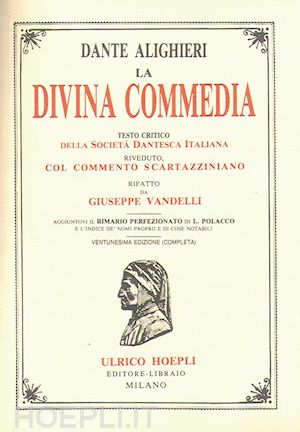
\includegraphics[scale=0.2]{images/divina.jpg}};
    			\node (c) [below=of b, yshift=0.5cm] {
\includegraphics[scale=0.07]{images/film.jpg}};
    			
    			\begin{pgfonlayer}{background}
    			\node[bigbox] [fit = (a) (c)] {};
    			\end{pgfonlayer}
    			
    			\node[xshift=3.4cm] (title2) [draw, right=of title1] {Output};
    			
    			\node (d) [draw, right=of a, xshift = 0.5cm] {52c61456bd3d60c08599a8c61e113e7b \\ c39118b75d06b2643c55957ece91269b};
    			\node (e) [draw, right=of b, xshift=0.7cm] {1f12f8384d5941e8e273926635be646a \\ f786405a8662e0ba6dd1fd0526ec0528};
    			\node (f) [draw, right=of c, xshift=0.3cm] {721a14d89cb463b51cf20ecc707aa290 \\ 5b7c8f32d9114dc19fe353e611494bf1};
    			
    			\begin{pgfonlayer}{background}
    			\node[bigbox] [fit = (d) (f)] {};
    			\end{pgfonlayer}
    			

    			\node[xshift=1.9cm, yshift=-1.2cm] (z) {$\xrightarrow{\ \ \ \ \ \ \ \ \ \ \ }{}$};
    			\node[xshift=1.8cm, yshift=-1.5cm] (z) {$\NOT{\xleftarrow{\ \ \ \ \ \ \ \ \ \ \ }}{}$};
    			\node[xshift=1.8cm, yshift=-3.4cm] (z) {$\xrightarrow{\ \ \ \ \ \ \ \ \ \ \ \ }{}$};
    			\node[xshift=1.7cm, yshift=-3.7cm] (z) {$\NOT{\xleftarrow{\ \ \ \ \ \ \ \ \ \ \ \ }}{}$};
    			\node[xshift=2cm, yshift=-6.2cm] (z) {$\xrightarrow{\ \ \ \ \ \ \ \ \ }{}$};
    			\node[xshift=1.9cm, yshift=-6.5cm] (z) {$\NOT{\xleftarrow{\ \ \ \ \ \ \ \ \ }}{}$};

    			
    			\node (g) [right=of d, xshift = -0.9cm] {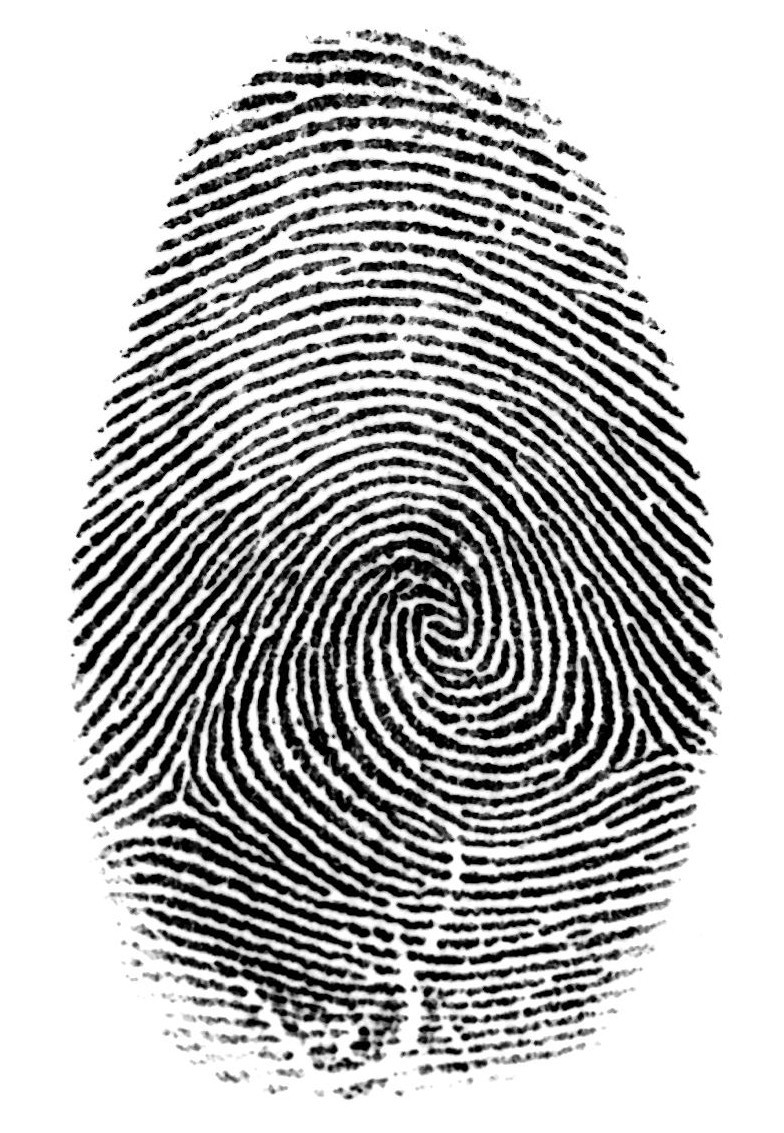
\includegraphics[scale=0.14]{images/fingerprint1.jpg}};
    			\node (g) [right=of e, xshift = -0.7cm] {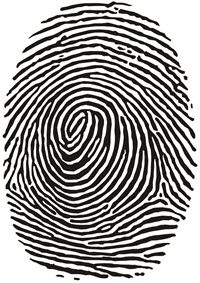
\includegraphics[scale=0.24]{images/fingerprint2.jpg}};
    			\node (g) [right=of f, xshift = -0.8cm] {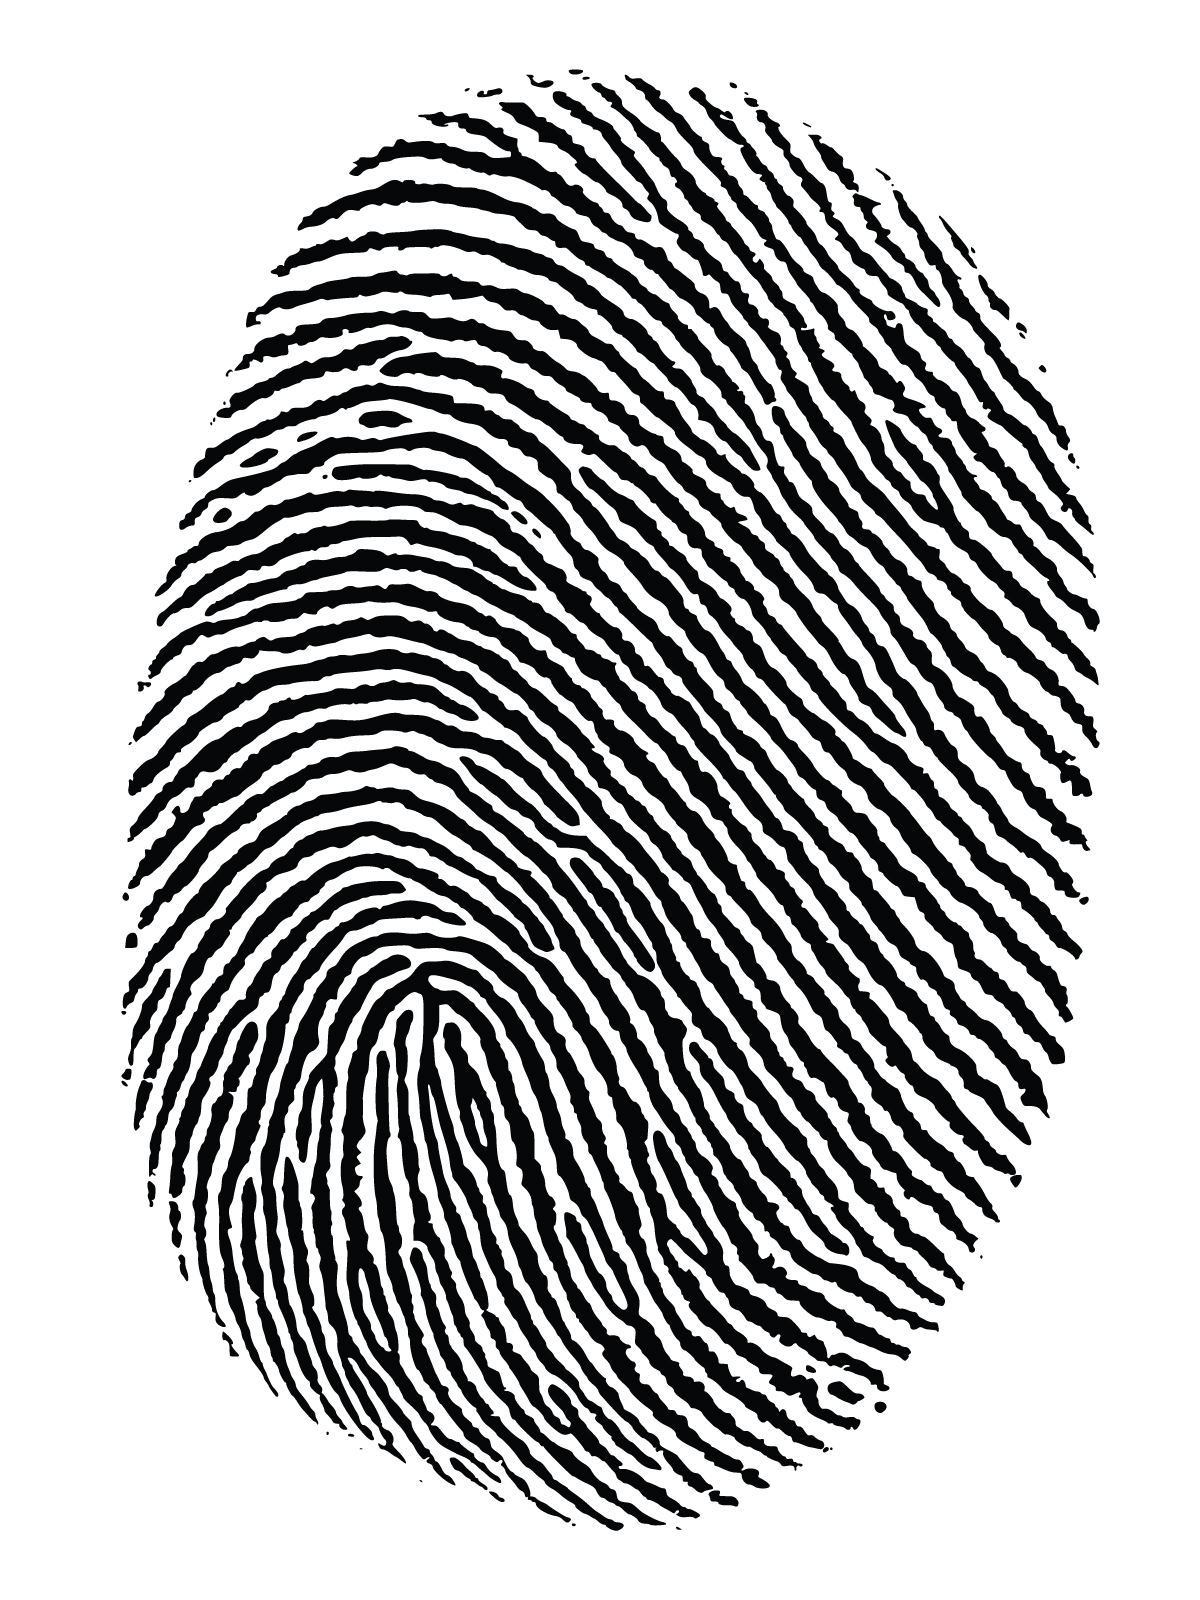
\includegraphics[scale=0.02]{images/fingerprint3.jpg}};
    			
    			\node (h) [right=of a, xshift = -0.7cm, yshift = 0.3cm] {\tiny SHA-256};
    			\node (h) [right=of b, xshift = -0.5cm, yshift = 0.3cm] {\tiny SHA-256};
    			\node (h) [right=of c, xshift = -0.95cm, yshift = 0.3cm] {\tiny SHA-256};
    			\end{tikzpicture}
    		\end{center}
		\end{frame}

		\subsection{Elliptic curve cryptography}
		\begin{frame}{Elliptic curve cryptography}
			\begin{columns}
				\begin{column}{0.5\linewidth}
					An elliptic curve over a finite field is defined by: 
					$$E(\mathbb{F}_p): \ y^2 = x^3 + ax + b \ (\text{mod} \ p).$$
					It is possible to define:
					\begin{itemize}
						\item<2 -> Addition: \\
						$Q_3 := Q_1 + Q_2, \ \forall Q_1, Q_2 \in E(\mathbb{F}_p)$;
						\item<3 -> Scalar multiplication: \\
						$nG = G + ... + G$, $\forall G \in E(\mathbb{F}_p),$ $\forall n \in \mathbb{N}$.
					\end{itemize}
				\onslide<4>{Multiplication's computational asymmetry is the core of ECC.}
			\end{column}
			\begin{column}{0.6\linewidth}
				\begin{tikzpicture}[
					every node/.style = {% is not necessary, default node's shape is rectangle
					align=center}
					]
				
					\node () at (0,0) {};
					\node (a) [xshift = 2.3cm] {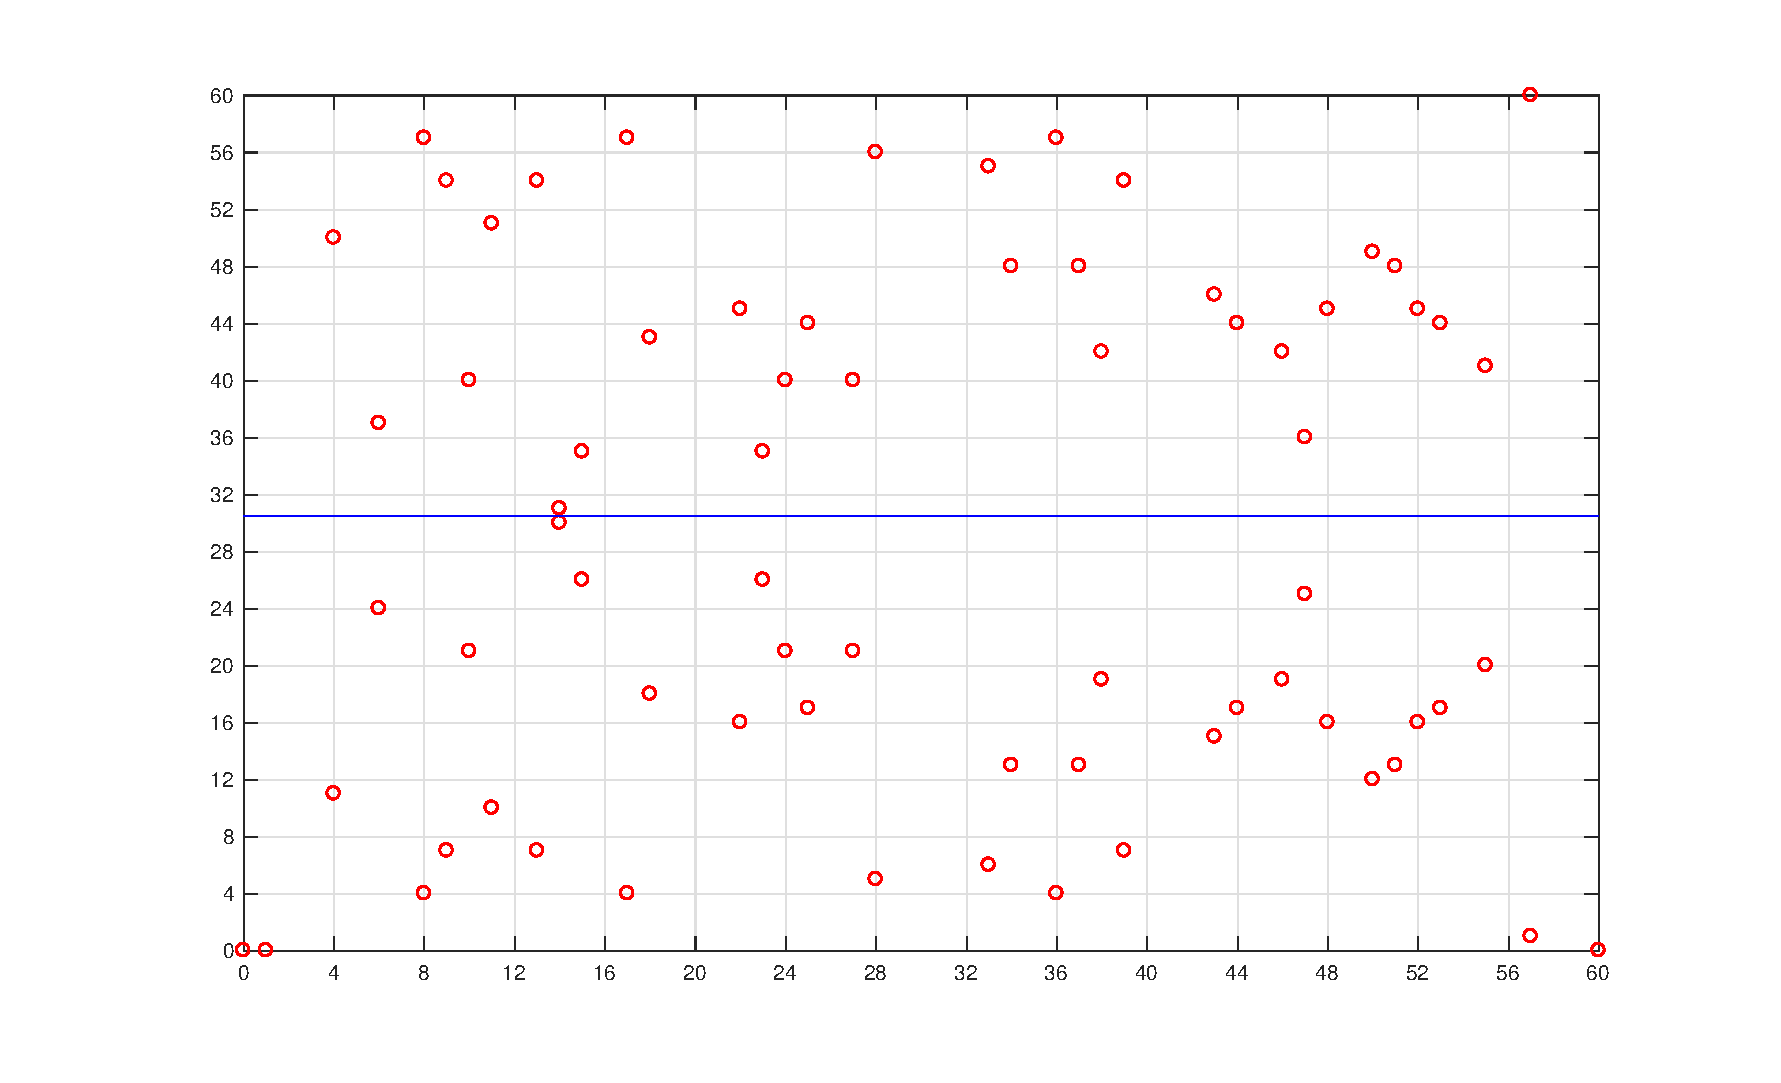
\includegraphics[height=5cm, width=6.4cm]{images/ec_over_ff}};
				
					\node (b) [below=of a, yshift = 1.2cm] {\small The curve $y^2 = x^3 - x \ \text{over} \ \mathbb{F}_{61}$.};
				\end{tikzpicture}
			\end{column}
		\end{columns}
	\end{frame}

    
    \begin{frame}{Discrete logarithm problem}
    	Fixed $G \in E(\mathbb{F}_p)$, we can define $Q = qG \ \ \forall q \in [1, ..., n - 1]$:
    	\begin{itemize}
    		\item<2-> The direct operation $q \mapsto Q$ is efficient;
    		\item<3-> The inverse operation $Q \mapsto q$ is computationally infeasible for certain groups.
    	\end{itemize}
    	
    	\onslide<4->{Asymmetric cryptography: $\{q, Q\}$ is a key pair whose elements have complementary roles.}

		\bigskip
		
		\onslide<5>{
	 	\begin{block}{Double and add algorithm: $q = 41$}
			$$41 = 1 + 8 + 32  \ \Longrightarrow \ 41G = G + 8G + 32G.$$
		
			\noindent
			5 point doubling and 2 additions vs. 40 additions.
		\end{block}}
	\end{frame}
    
    \section{Digital signature schemes}
    
    \begin{frame}{Digital signature}
        \begin{center}
        	\begin{tikzpicture}[
        	every node/.style = {% is not necessary, default node's shape is rectangle
        		align=center}
        	]
        	
        	\node (a) {
\includegraphics[scale=0.2]{images/Alice.jpg}};
        	\node (b) [text width=3cm, below=of a, yshift=1cm] {Alice};
        	
        	\node (d) [right=of a] {
\includegraphics[scale=0.25]{images/Bob.jpg}};
        	\node (e) [text width=3cm, below=of d, yshift=1cm] {Bob};
        	
        	\node<1-4> (c) [xshift=2.1 cm, yshift=-1cm] {
\includegraphics[scale=0.1]{images/sig.jpg}};
        	\node<1> (f) [xshift = 2.1 cm, yshift = 1cm] {
\includegraphics[scale=0.06]{images/doc.png}};
        	\node<2-> (f) [xshift = 2.1 cm, yshift = 1cm] {
\includegraphics[scale=0.1]{images/bitcoin.png}};
        	\node<5> (c) [xshift=2.1 cm, yshift=-1cm] {
\includegraphics[scale=0.1]{images/bitcoin_sig.jpg}};

        	
        	\node<3> (f) [xshift = -1.2 cm, yshift = 1cm] {$q_A$};
        	\node<3> (f) [xshift = 5.5 cm, yshift = 1cm] {$Q_A$};
        	\node<4-> (f) [xshift = -1.2 cm, yshift = 1cm] {\textcolor{red}{$q_A$}};
        	\node<4-> (f) [xshift = 5.5 cm, yshift = 1cm] {\textcolor{green}{$Q_A$}};
        	
        	
        	
        	
        	\draw [->] (a) -- (d);
        	\end{tikzpicture}
        	\begin{itemize}
        		\item<3-> Authentication: the recipient is confident that the message comes from the alleged sender;
        		\item<4-> Non repudiation: the sender cannot deny having sent the message;
        		\item<5> Integrity: ensures that the message has not been altered during transmission.
        	\end{itemize}
        \end{center}
    \end{frame}

	\subsection{ECDSA}
	\begin{frame}{Elliptic curve digital signature algorithm}
		\begin{columns}
			\begin{column}{0.6\linewidth}
				ECDSA\_SIG$(m, q)$:
				\begin{enumerate}
					\item<3 -> $z \gets \text{hash}(m)$;
					\item<4 -> $k \xleftarrow{\text{\$}} \{1, ..., n - 1\}$;
					\item<5 -> $K \gets kG$;
					\item<6 -> $r \gets x_K \ (\text{mod} \ n)$;
					\item<7 -> $s \gets k^{-1}(z + rq) \ (\text{mod} \ n)$;
					\item<8 -> \textbf{return} $(r, s)$.
				\end{enumerate}
			\end{column}
			\begin{column}{0.5\linewidth}
				\begin{figure}
				\only<1> {\vspace*{-0.7cm}
					\hspace*{-1.7cm}
					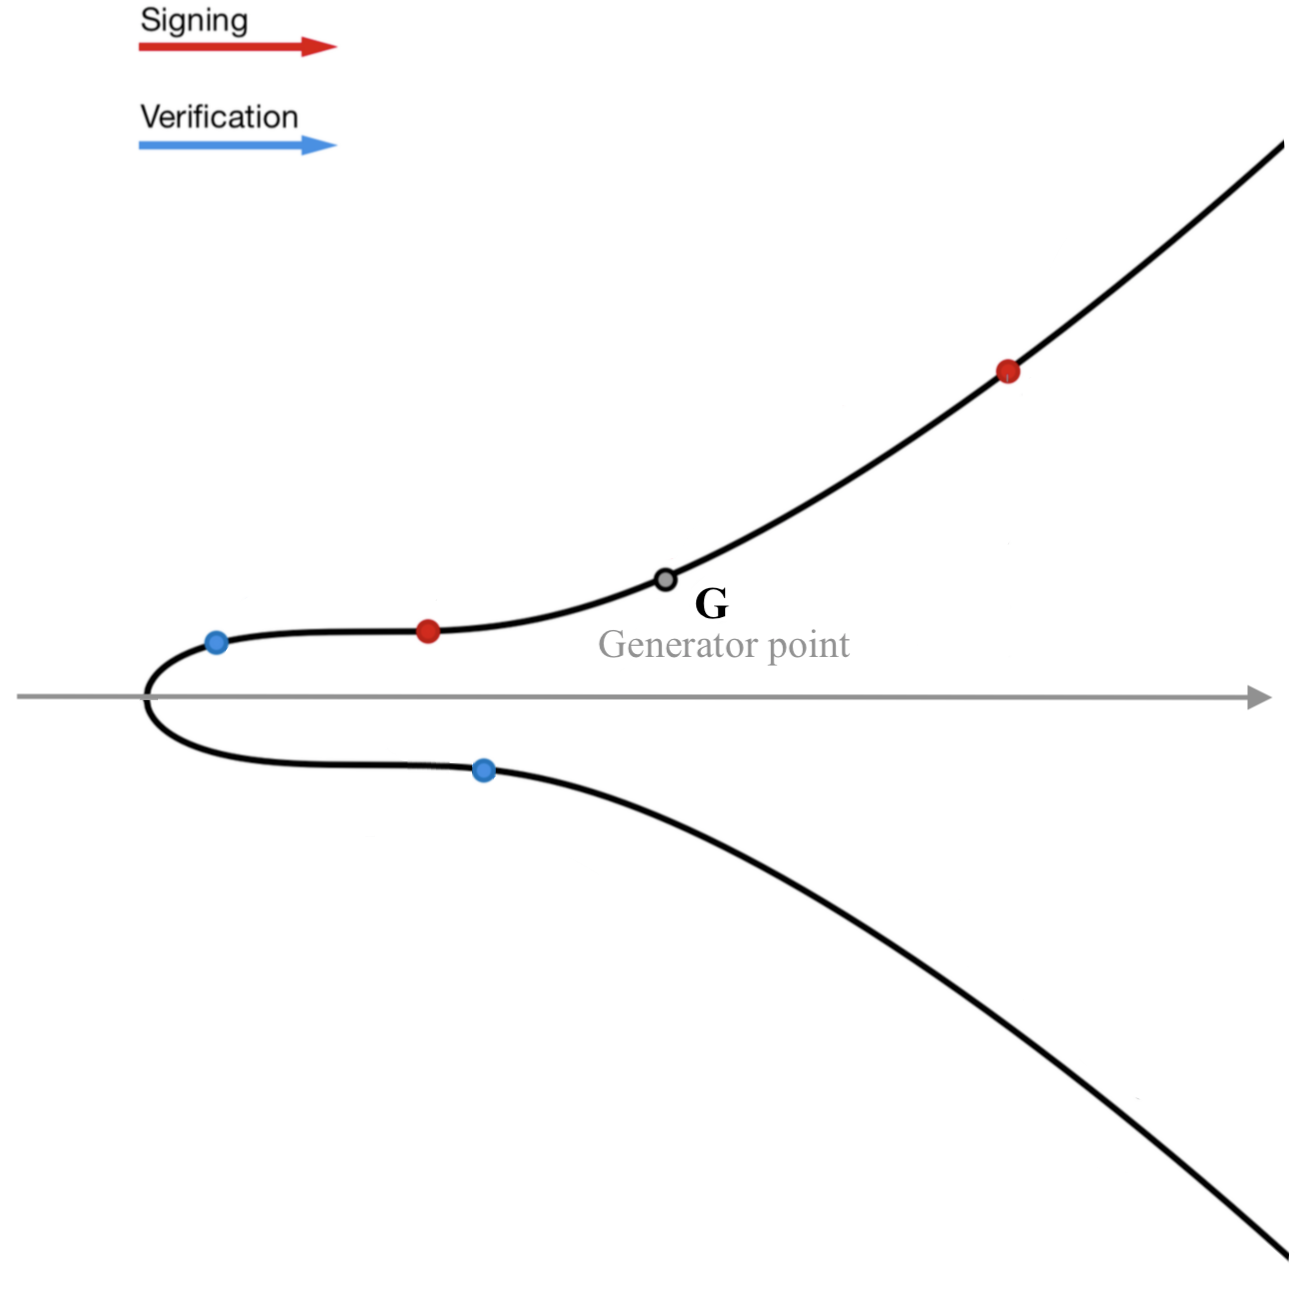
\includegraphics[scale=0.29]{images/ECDSA1}
				\source{\tiny \url{https://medium.com/cryptoadvance/how-schnorr-signatures-may-improve-bitcoin-91655bcb4744}}}
				\only<2-4> {\vspace*{-0.7cm}
					\hspace*{-1.7cm}
					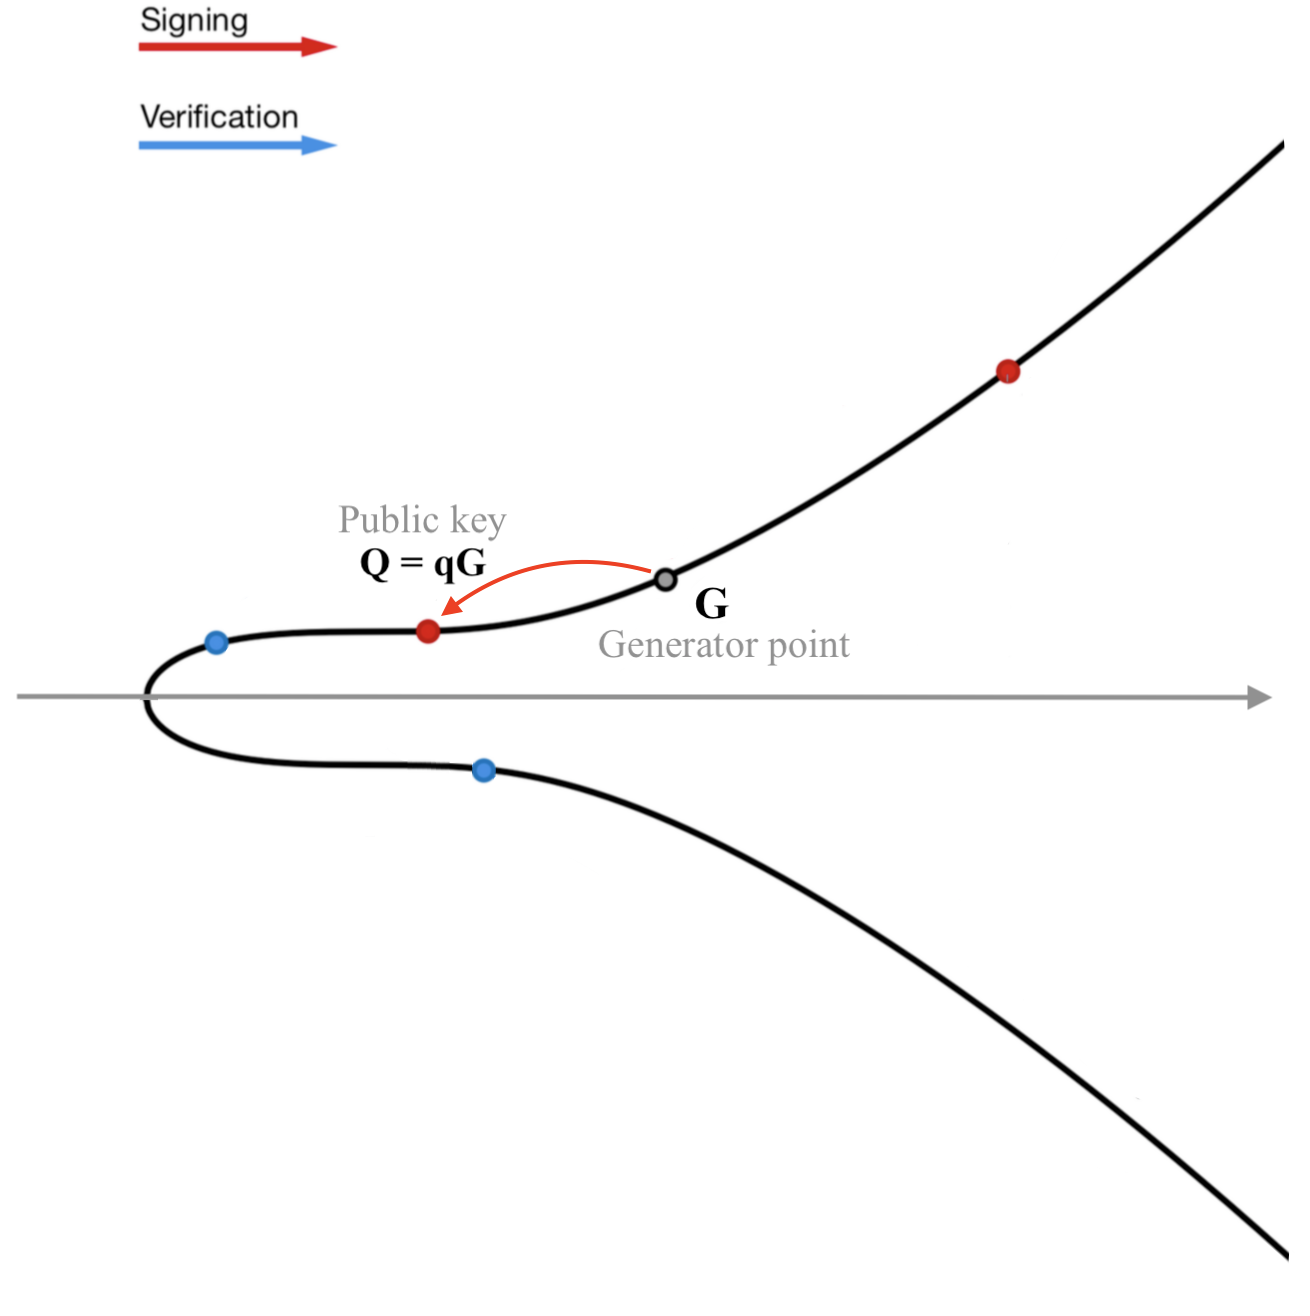
\includegraphics[scale=0.29]{images/ECDSA2}
				\source{\tiny \url{https://medium.com/cryptoadvance/how-schnorr-signatures-may-improve-bitcoin-91655bcb4744}}}
				\only<5> {\vspace*{-0.7cm}
					\hspace*{-1.7cm}
					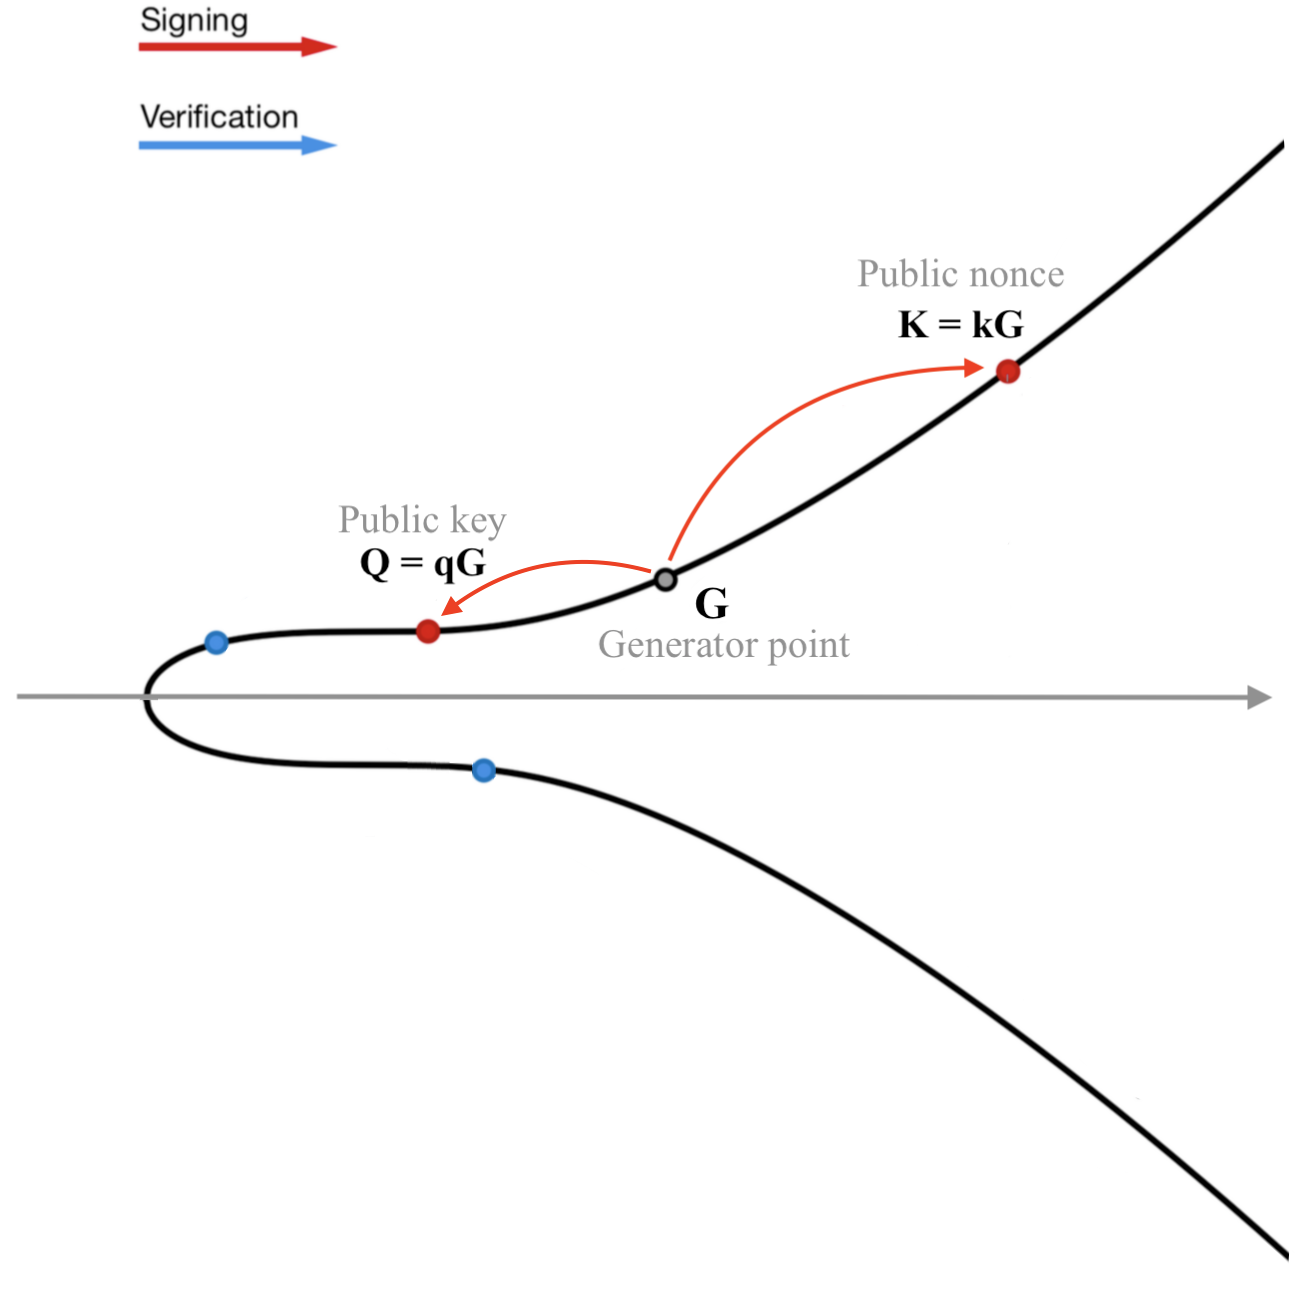
\includegraphics[scale=0.29]{images/ECDSA3}
				\source{\tiny \url{https://medium.com/cryptoadvance/how-schnorr-signatures-may-improve-bitcoin-91655bcb4744}}}
				\only<6-8> {\vspace*{-0.7cm}
					\hspace*{-1.7cm}
					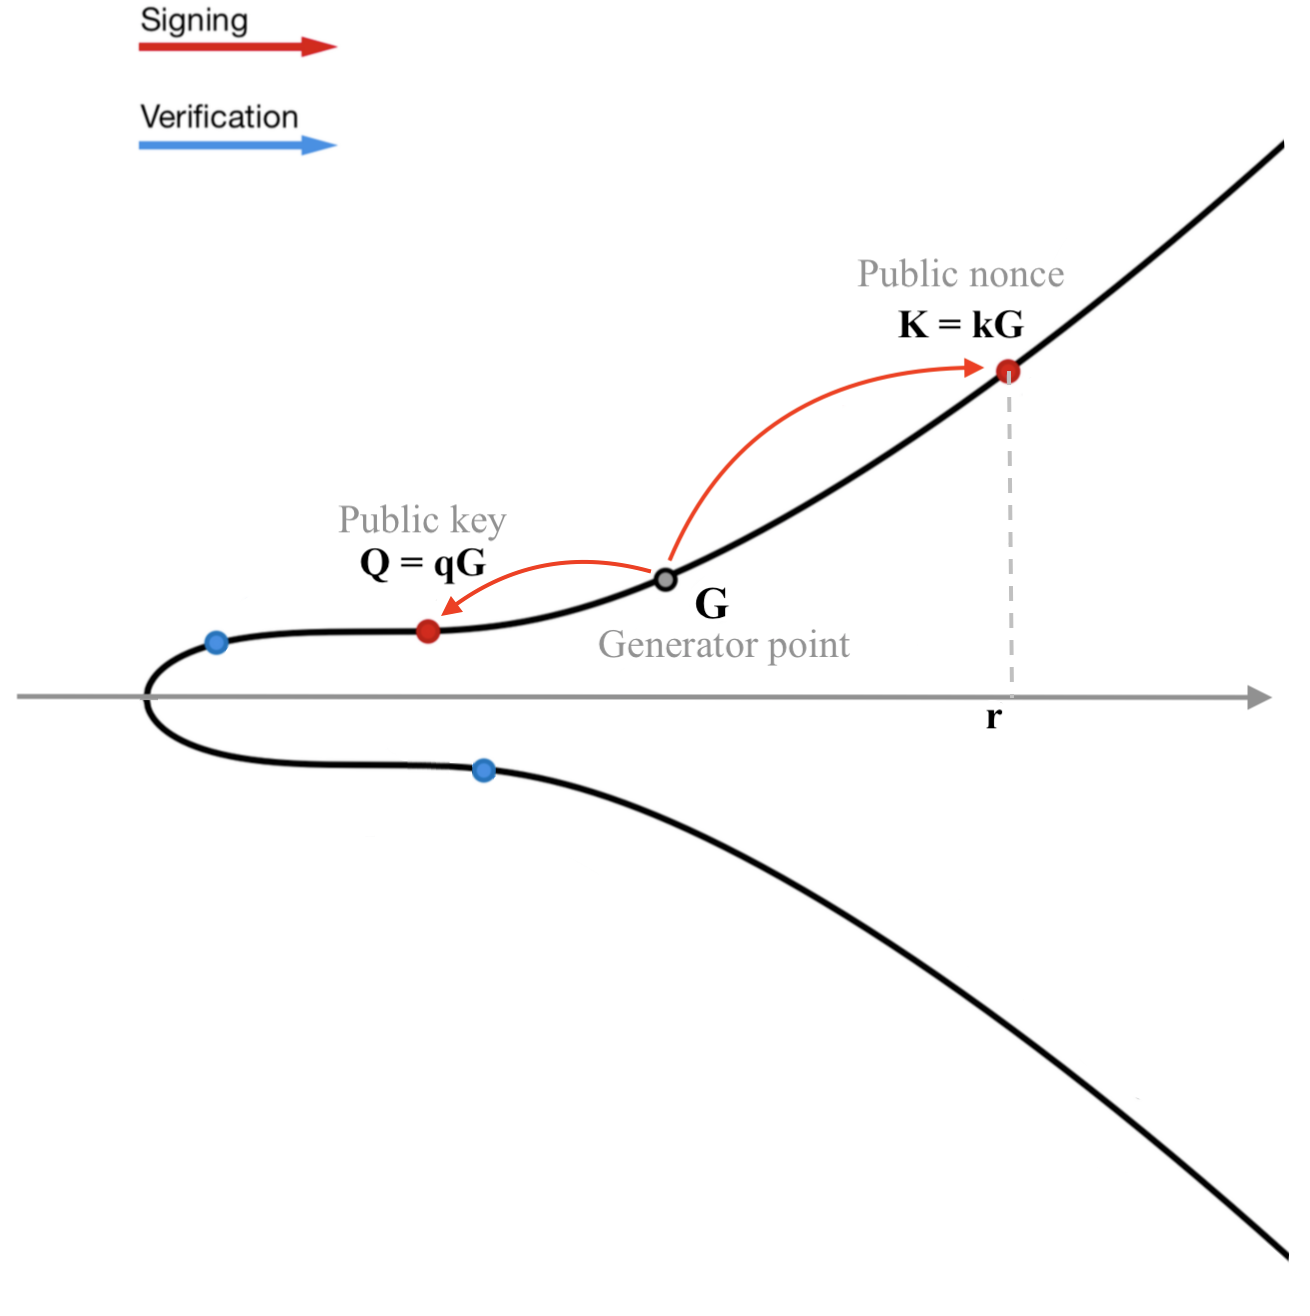
\includegraphics[scale=0.29]{images/ECDSA4}
				\source{\tiny \url{https://medium.com/cryptoadvance/how-schnorr-signatures-may-improve-bitcoin-91655bcb4744}}}
				\end{figure}
			\end{column}
		\end{columns}
	\end{frame}

	\begin{frame}{Elliptic curve digital signature algorithm}
		\begin{columns}
			\begin{column}{0.6\linewidth}
				ECDSA\_VER$((r,s), m, Q)$:
				\begin{enumerate}
					\item<2 -> \textbf{If} $r \notin \{1, ..., n - 1\}$ \textbf{or} $s \notin \{1, ..., n - 1\}$: \\ \textbf{\ \ \ return False};
					\item<3 -> $z \gets \text{hash}(m)$;
					\item<4 -> $u_1 \gets zs^{-1} \ (\text{mod} \ n)$, $u_2 \gets rs^{-1} \ (\text{mod} \ n)$;
					\item<5 -> $K \gets u_1G + u_2Q$;
					\item<7 -> \textbf{return $r = x_K \ (\text{mod} \ n)$}.
				\end{enumerate}
			\end{column}
			\begin{column}{0.5\linewidth}
				\begin{figure}
					\only<1-3> {\vspace*{-0.7cm}
						\hspace*{-1.7cm}
						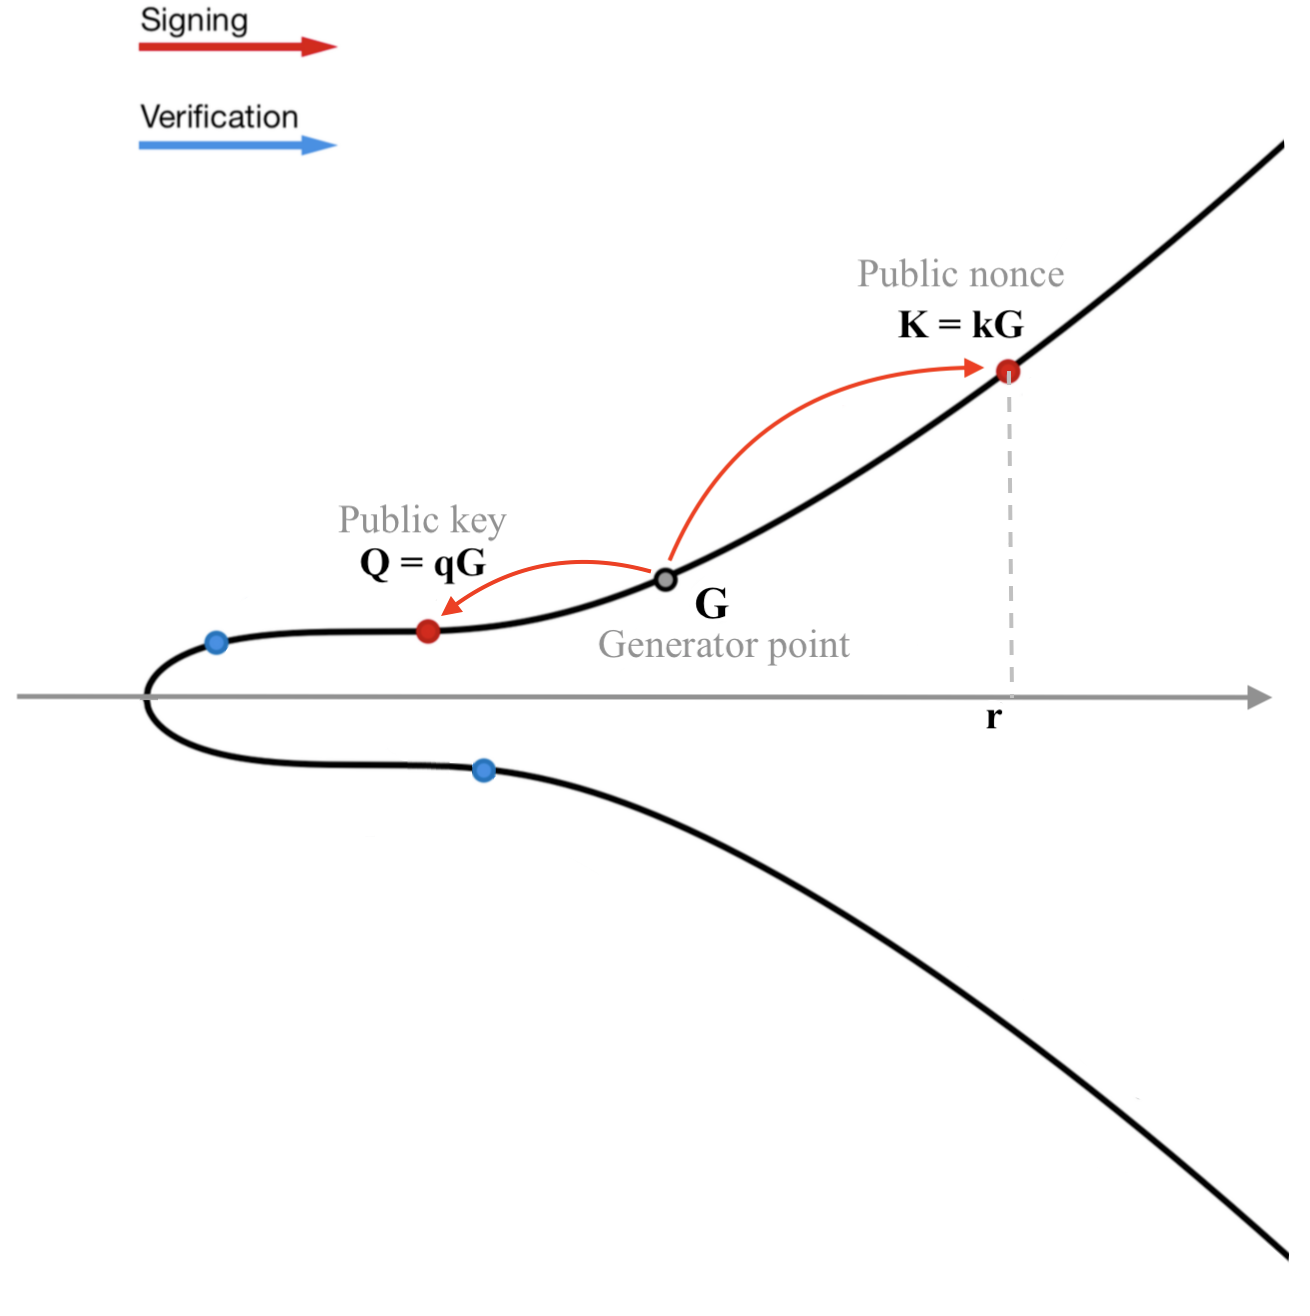
\includegraphics[scale=0.29]{images/ECDSA4}
						\source{\tiny \url{https://medium.com/cryptoadvance/how-schnorr-signatures-may-improve-bitcoin-91655bcb4744}}}
					\only<4> {\vspace*{-0.7cm}
						\hspace*{-1.7cm}
						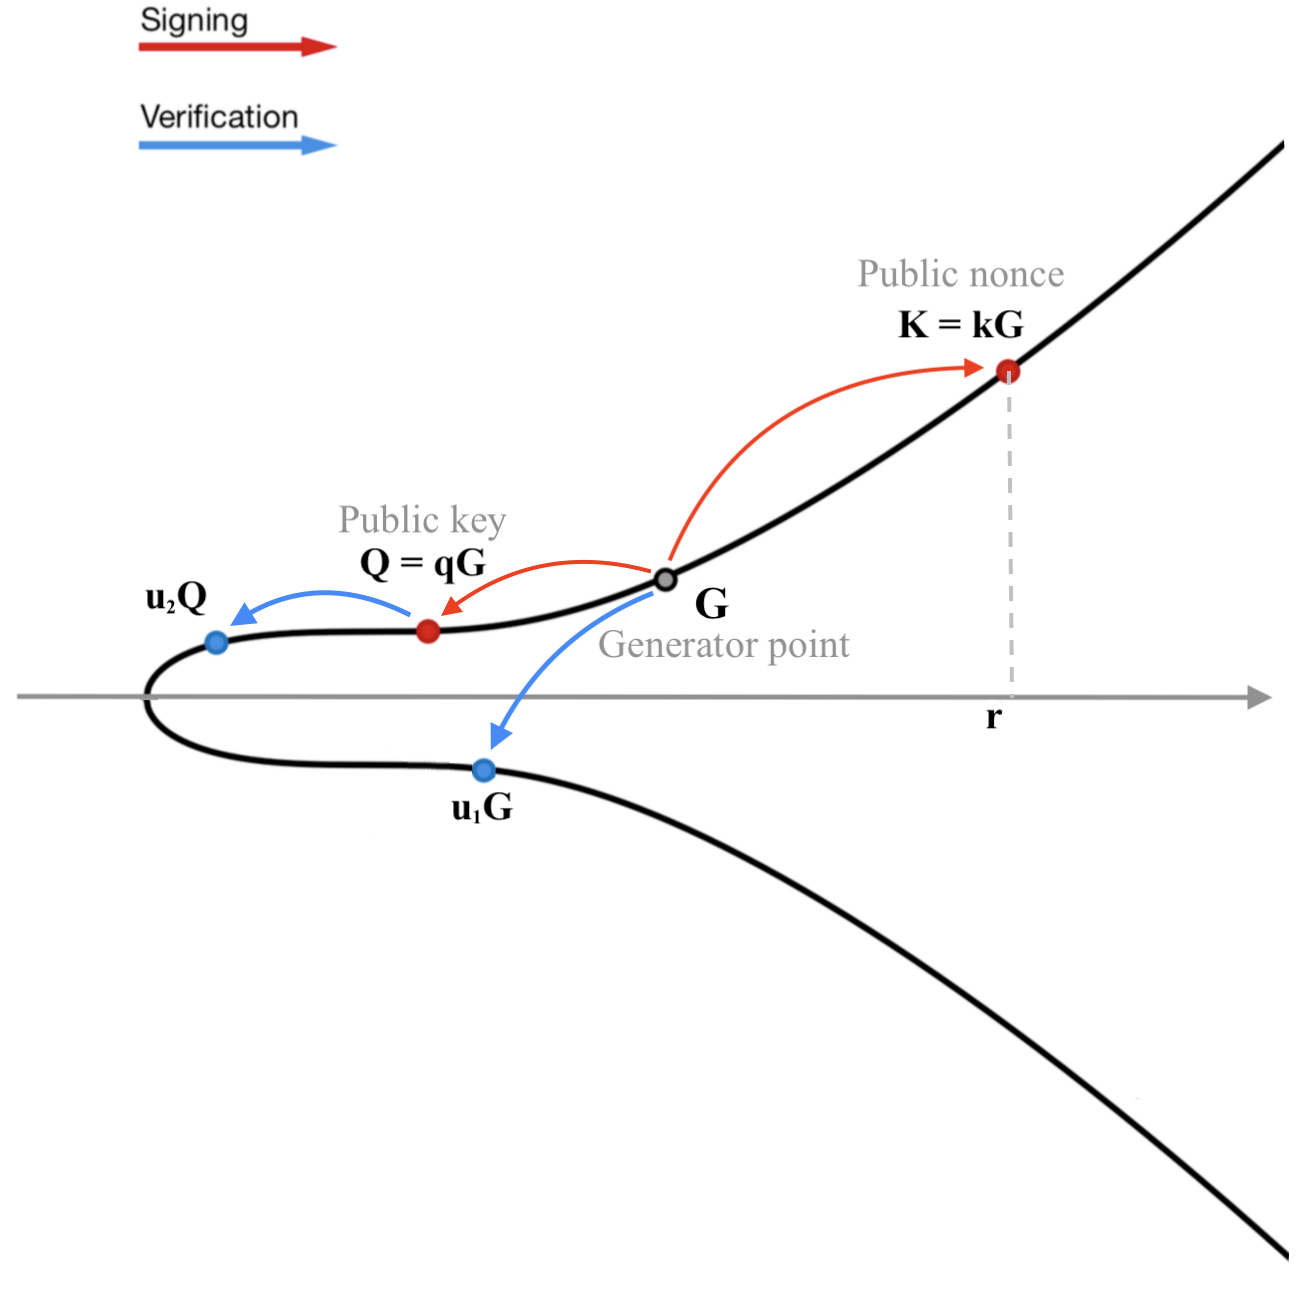
\includegraphics[scale=0.29]{images/ECDSA5}
						\source{\tiny \url{https://medium.com/cryptoadvance/how-schnorr-signatures-may-improve-bitcoin-91655bcb4744}}}
					\only<5> {\vspace*{-0.7cm}
						\hspace*{-1.7cm}
						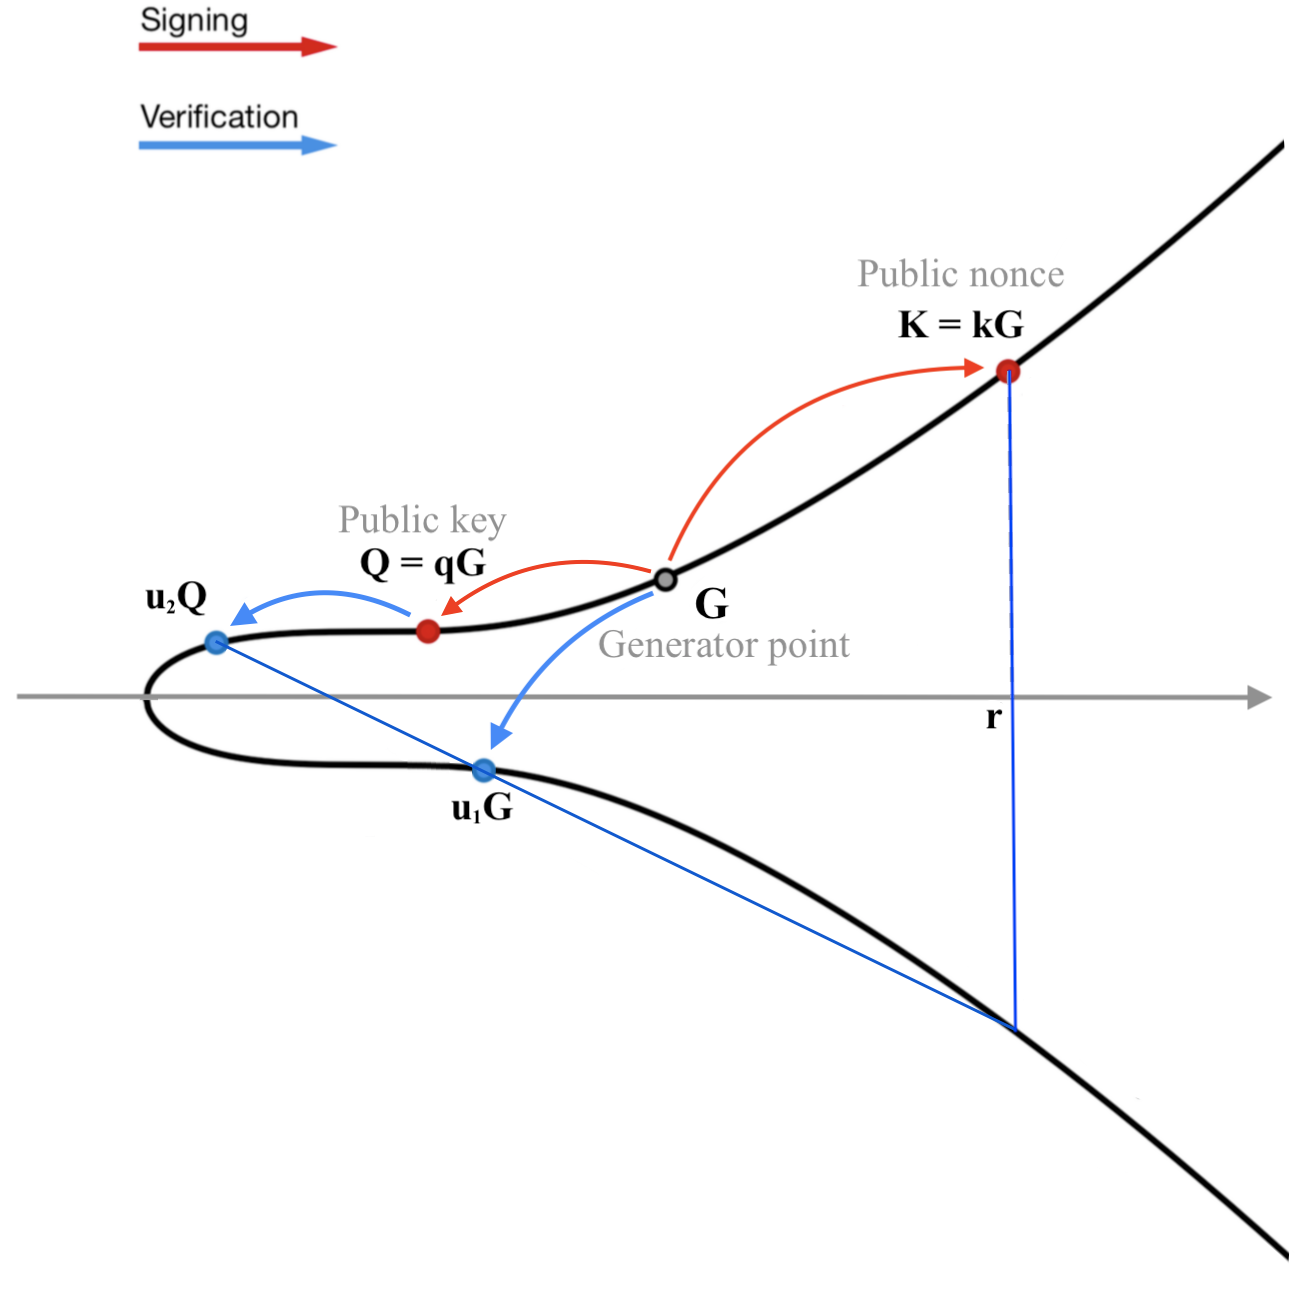
\includegraphics[scale=0.29]{images/ECDSA6}
						\source{\tiny \url{https://medium.com/cryptoadvance/how-schnorr-signatures-may-improve-bitcoin-91655bcb4744}}}
					\only<6-7> {\vspace*{-0.7cm}
						\hspace*{-1.7cm}
						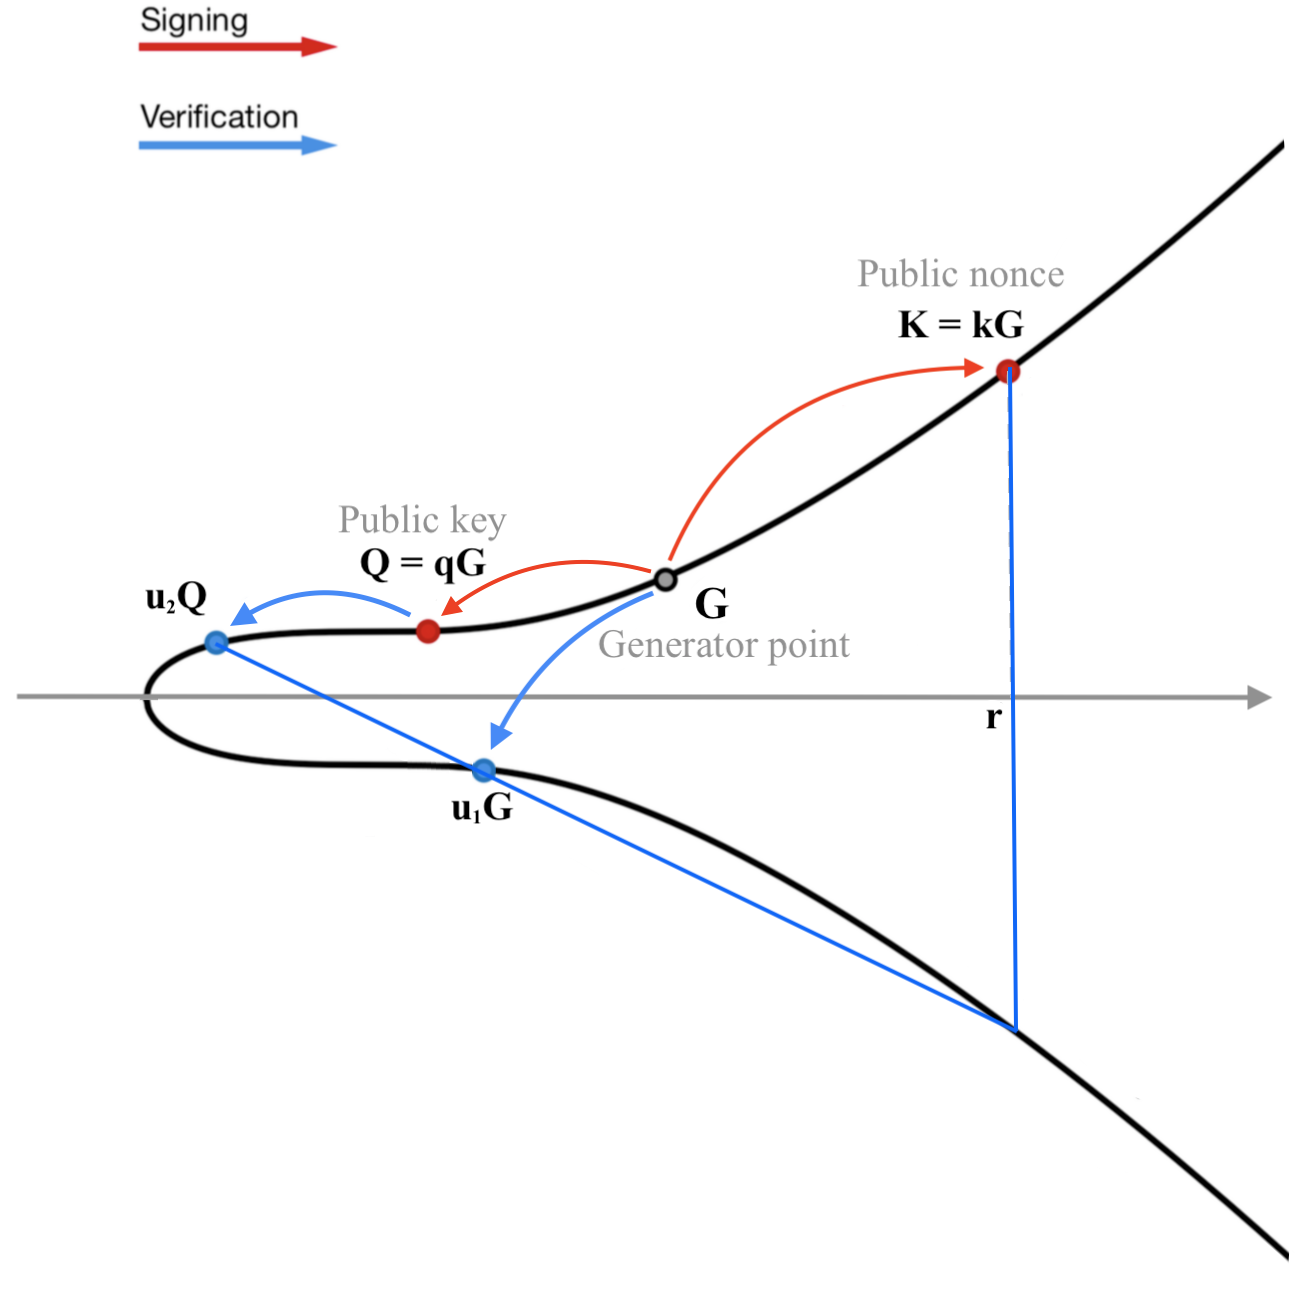
\includegraphics[scale=0.29]{images/ECDSA7}
						\source{\tiny \url{https://medium.com/cryptoadvance/how-schnorr-signatures-may-improve-bitcoin-91655bcb4744}}}
				\end{figure}
			\end{column}
		\end{columns}
	\end{frame}
	
	\subsection{ECSSA}
	\begin{frame}{Elliptic curve Schnorr signature algorithm}
		\begin{columns}
			\begin{column}{0.6\linewidth}
				ECSSA\_SIG$(m, q)$:
				\begin{enumerate}
					\item<3 -> $k \xleftarrow{\text{\$}} \{1, ..., n - 1\}$;
					\item<4 -> $K \gets kG$;
					\item<5 -> \textbf{If} $\text{jacobi}(y_K) \neq 1$: \\$\ \ \ k \gets n - k$;
					\item<6 -> $e \gets \text{hash}(x_K || qG || m) \ (\text{mod} \ n)$;
					\item<7 -> $s \gets k + eq \ (\text{mod} \ n)$;
					\item<8 -> \textbf{return} $(x_K, s)$.
				\end{enumerate}
			\end{column}
			\begin{column}{0.5\linewidth}
				\begin{figure}
					\only<1> {\vspace*{-0.7cm}
						\hspace*{-0.9cm}
						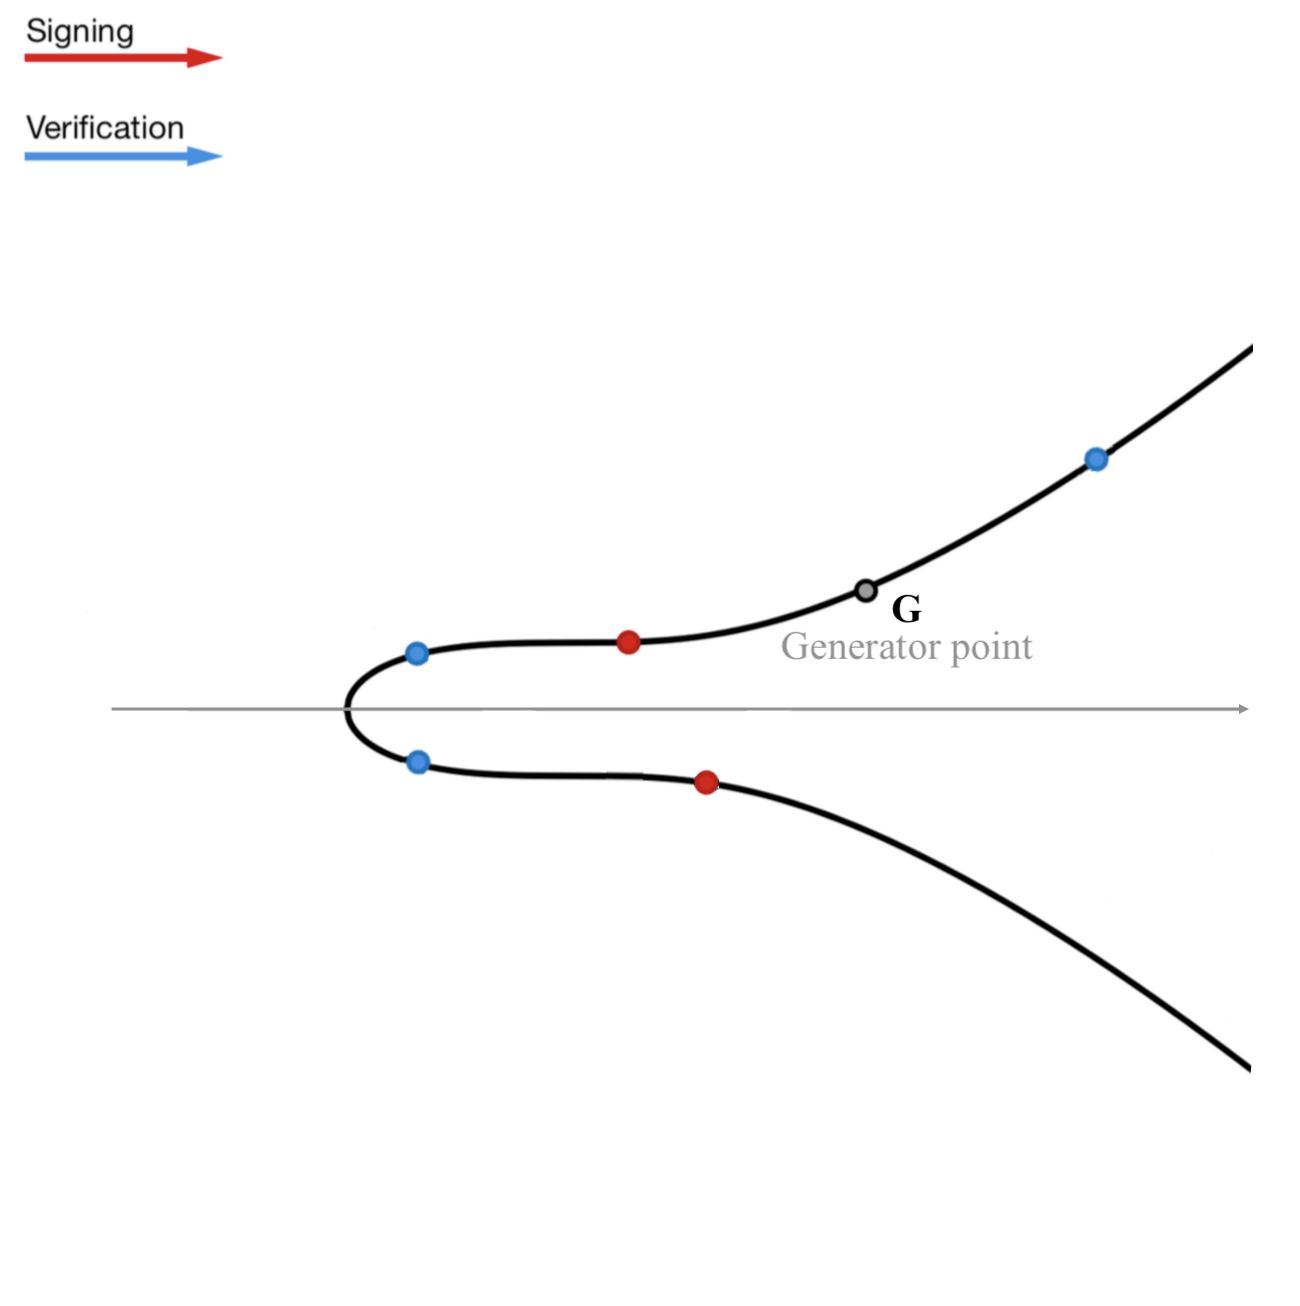
\includegraphics[scale=0.28]{images/Schnorr1}
						\source{\tiny \url{https://medium.com/cryptoadvance/how-schnorr-signatures-may-improve-bitcoin-91655bcb4744}}}
					\only<2-3> {\vspace*{-0.7cm}
						\hspace*{-0.9cm}
						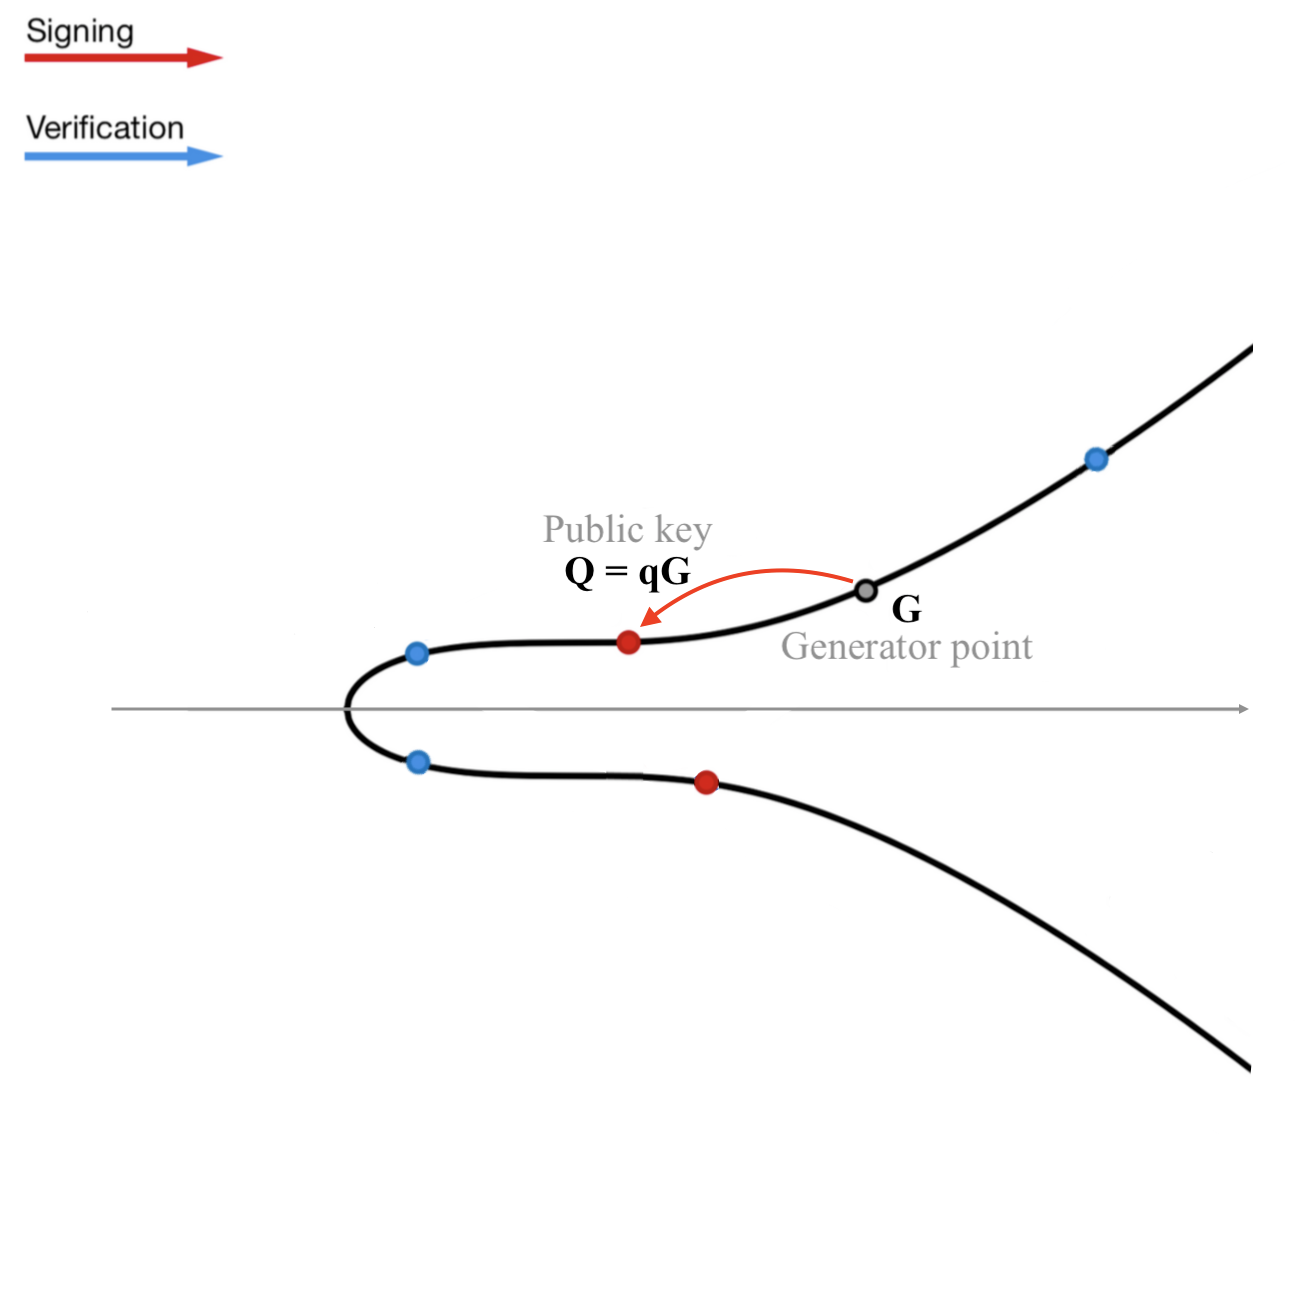
\includegraphics[scale=0.28]{images/Schnorr2}
						\source{\tiny \url{https://medium.com/cryptoadvance/how-schnorr-signatures-may-improve-bitcoin-91655bcb4744}}}
					\only<4> {\vspace*{-0.7cm}
						\hspace*{-0.9cm}
						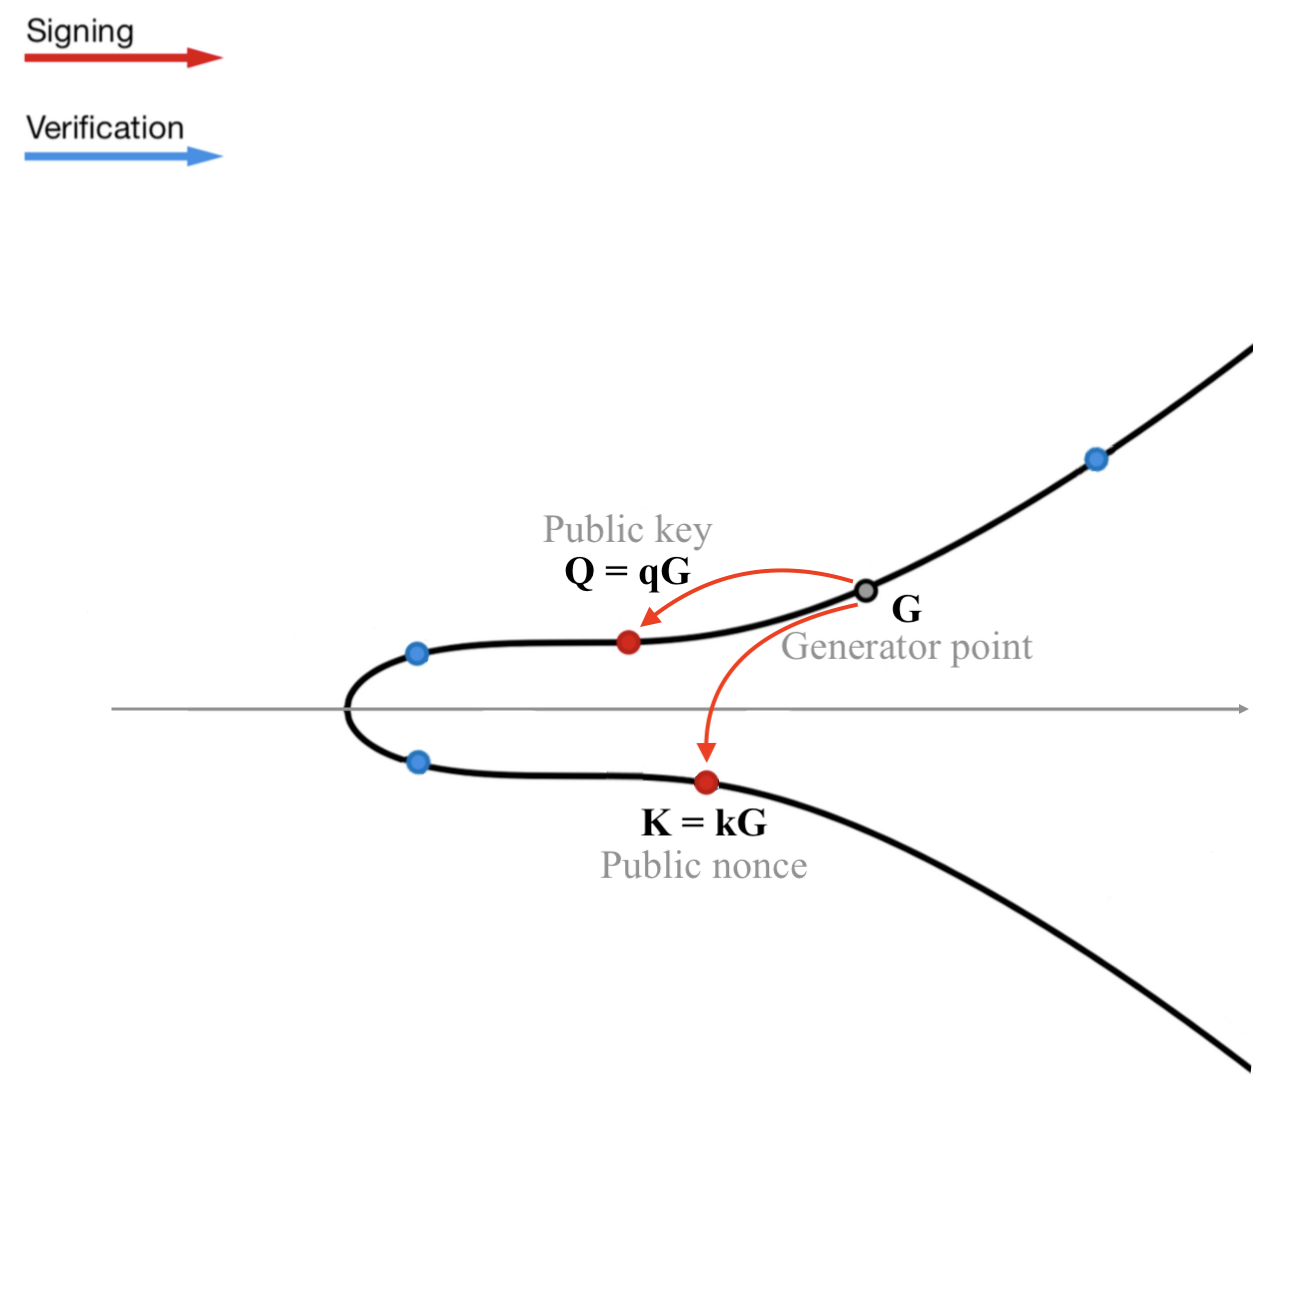
\includegraphics[scale=0.28]{images/Schnorr3}
						\source{\tiny \url{https://medium.com/cryptoadvance/how-schnorr-signatures-may-improve-bitcoin-91655bcb4744}}}
					\only<5> {\vspace*{-0.7cm}
						\hspace*{-0.9cm}
						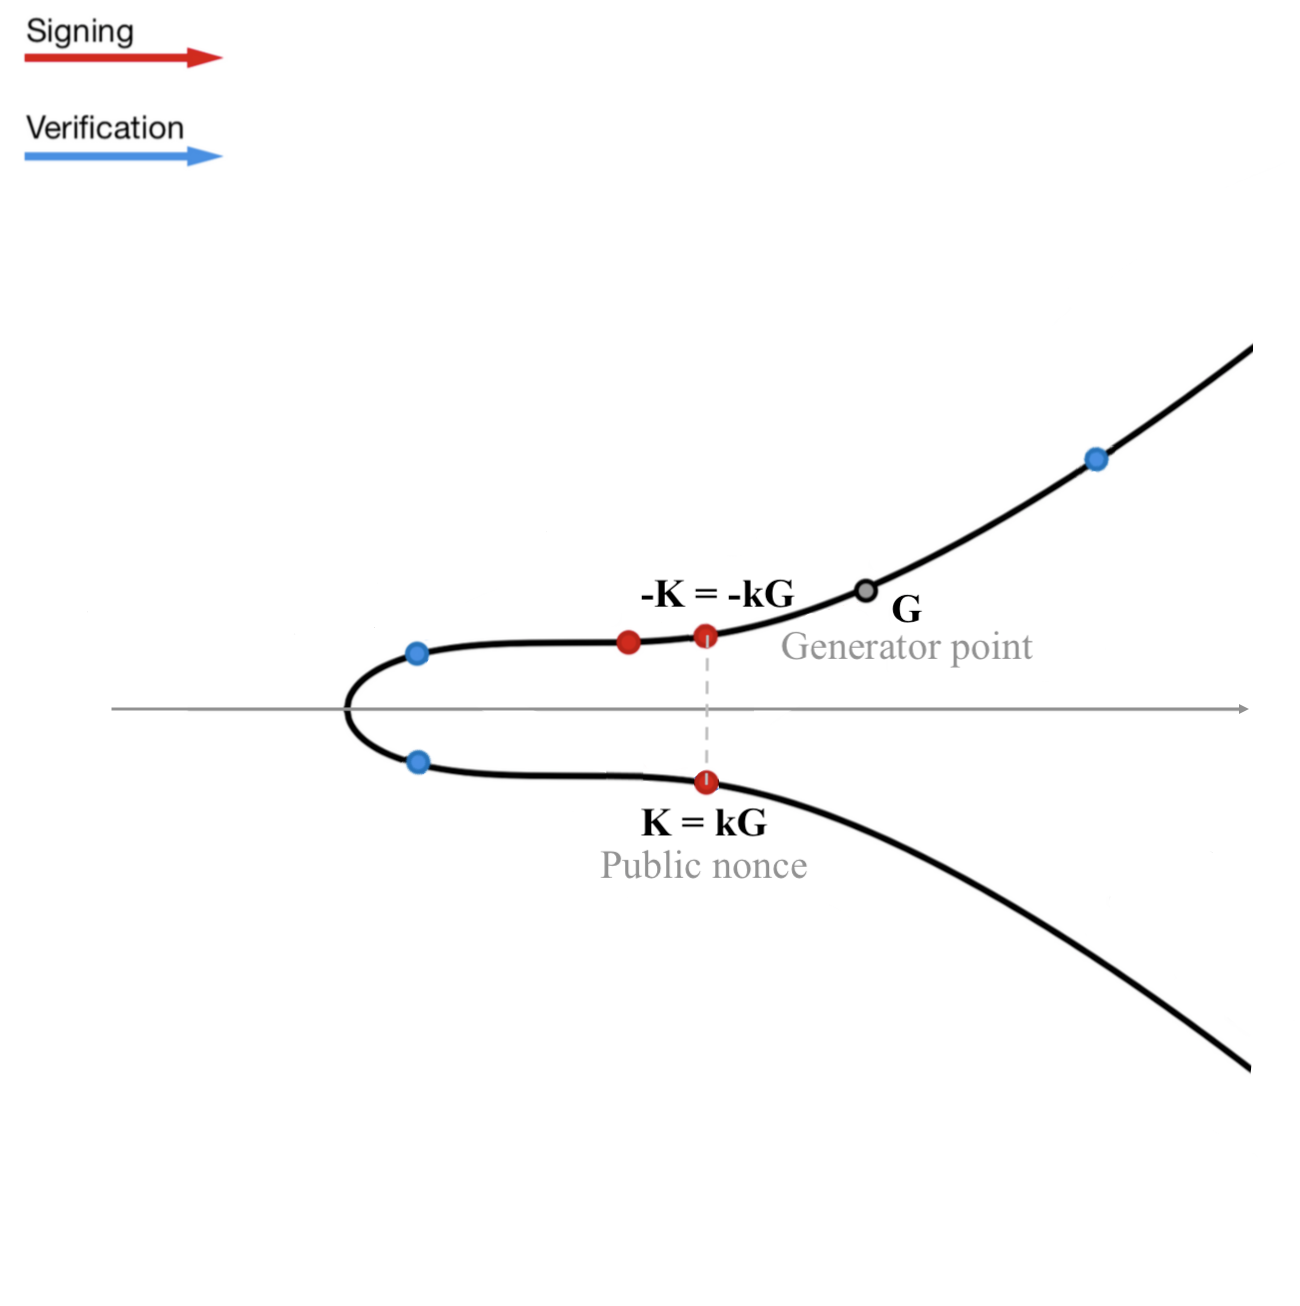
\includegraphics[scale=0.28]{images/Schnorr4}
						\source{\tiny \url{https://medium.com/cryptoadvance/how-schnorr-signatures-may-improve-bitcoin-91655bcb4744}}}
					\only<6-8> {\vspace*{-0.7cm}
						\hspace*{-0.9cm}
						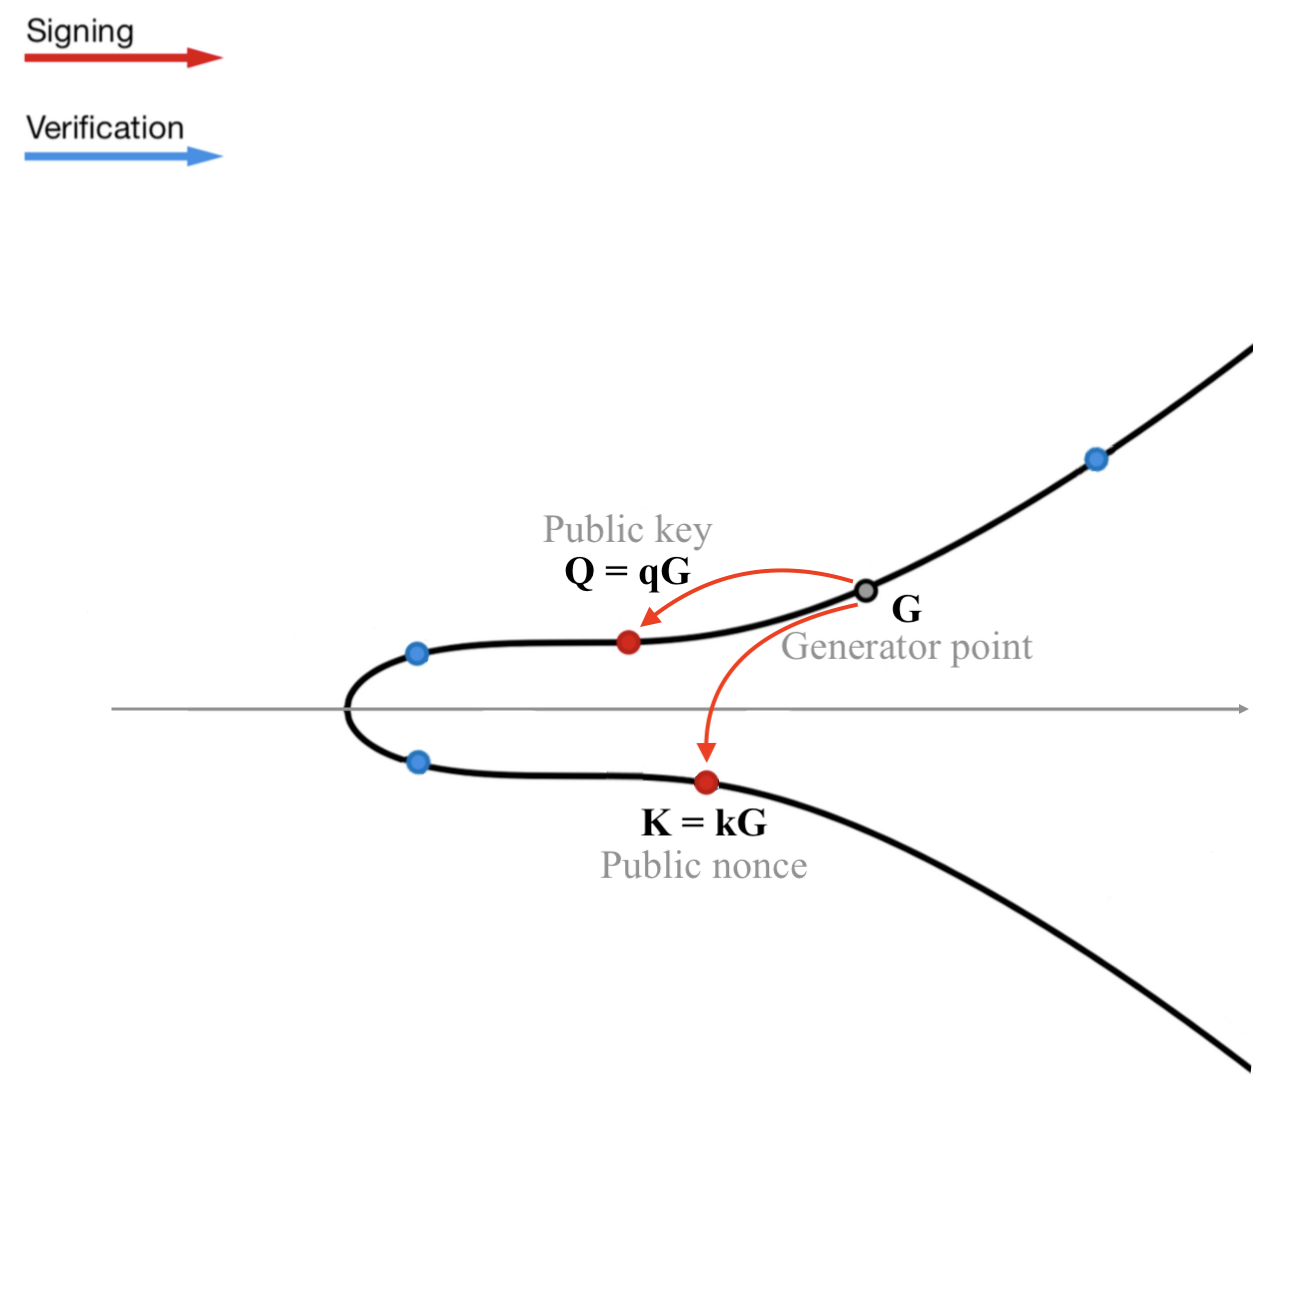
\includegraphics[scale=0.28]{images/Schnorr3}
						\source{\tiny \url{https://medium.com/cryptoadvance/how-schnorr-signatures-may-improve-bitcoin-91655bcb4744}}}
				\end{figure}
			\end{column}
		\end{columns}
	\end{frame}

	\begin{frame}{Elliptic curve Schnorr signature algorithm}
		\begin{columns}
			\begin{column}{0.6\linewidth}
				ECSSA\_VER$((r, s), m, Q)$:
				\begin{enumerate}
					\item<2 -> \textbf{If} $r \notin \{1, ..., p - 1\}$ or $s \notin \{1, ..., n - 1\}$: \\ \textbf{\ \ \ return False};
					\item<3 -> $e \gets \text{hash}(r || Q || m) \ (\text{mod} \ n)$;
					\item<4 -> $K \gets sG - eQ$;
					\item<8 -> \textbf{If} $\text{jacobi}(y_K) \neq 1$ \textbf{or} $x_K \neq r$: \\ \textbf{\ \ \ return False};
					\item<9 -> \textbf{return True}.
				\end{enumerate}
			\end{column}
			\begin{column}{0.5\linewidth}
				\begin{figure}
					\only<1-3> {\vspace*{-0.7cm}
						\hspace*{-0.9cm}
						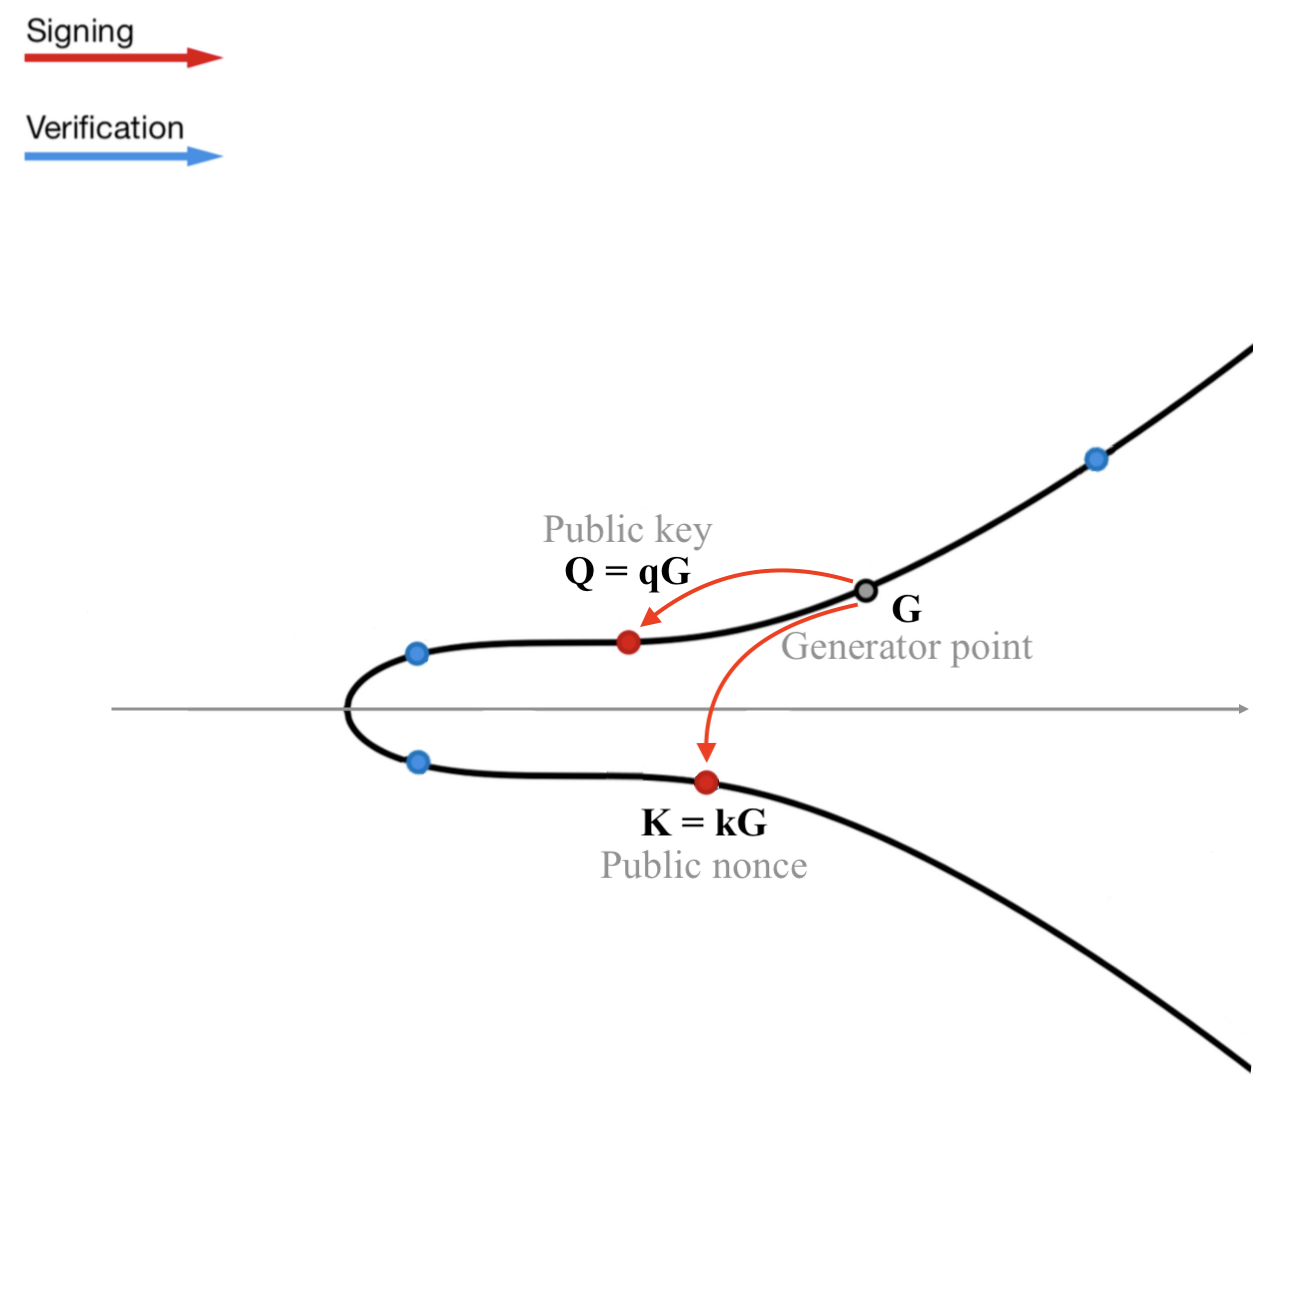
\includegraphics[scale=0.28]{images/Schnorr3}
						\source{\tiny \url{https://medium.com/cryptoadvance/how-schnorr-signatures-may-improve-bitcoin-91655bcb4744}}}
					\only<4> {\vspace*{-0.7cm}
						\hspace*{-0.9cm}
						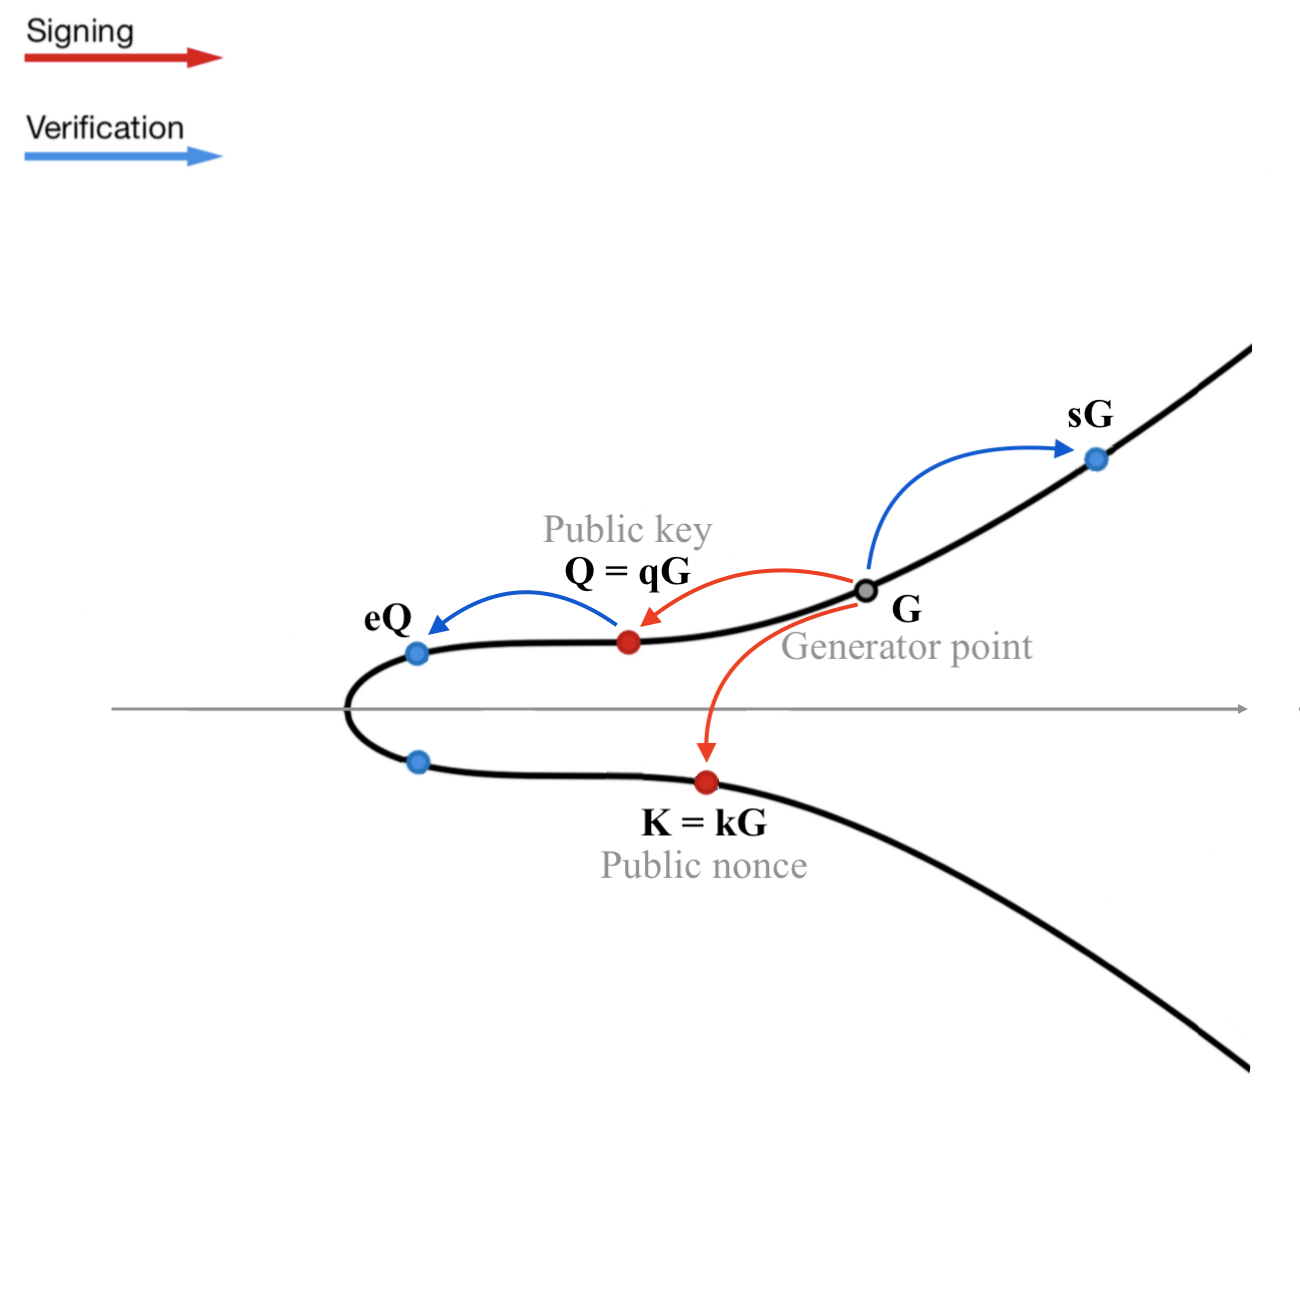
\includegraphics[scale=0.28]{images/Schnorr5}
						\source{\tiny \url{https://medium.com/cryptoadvance/how-schnorr-signatures-may-improve-bitcoin-91655bcb4744}}}
					\only<5> {\vspace*{-0.7cm}
						\hspace*{-0.9cm}
						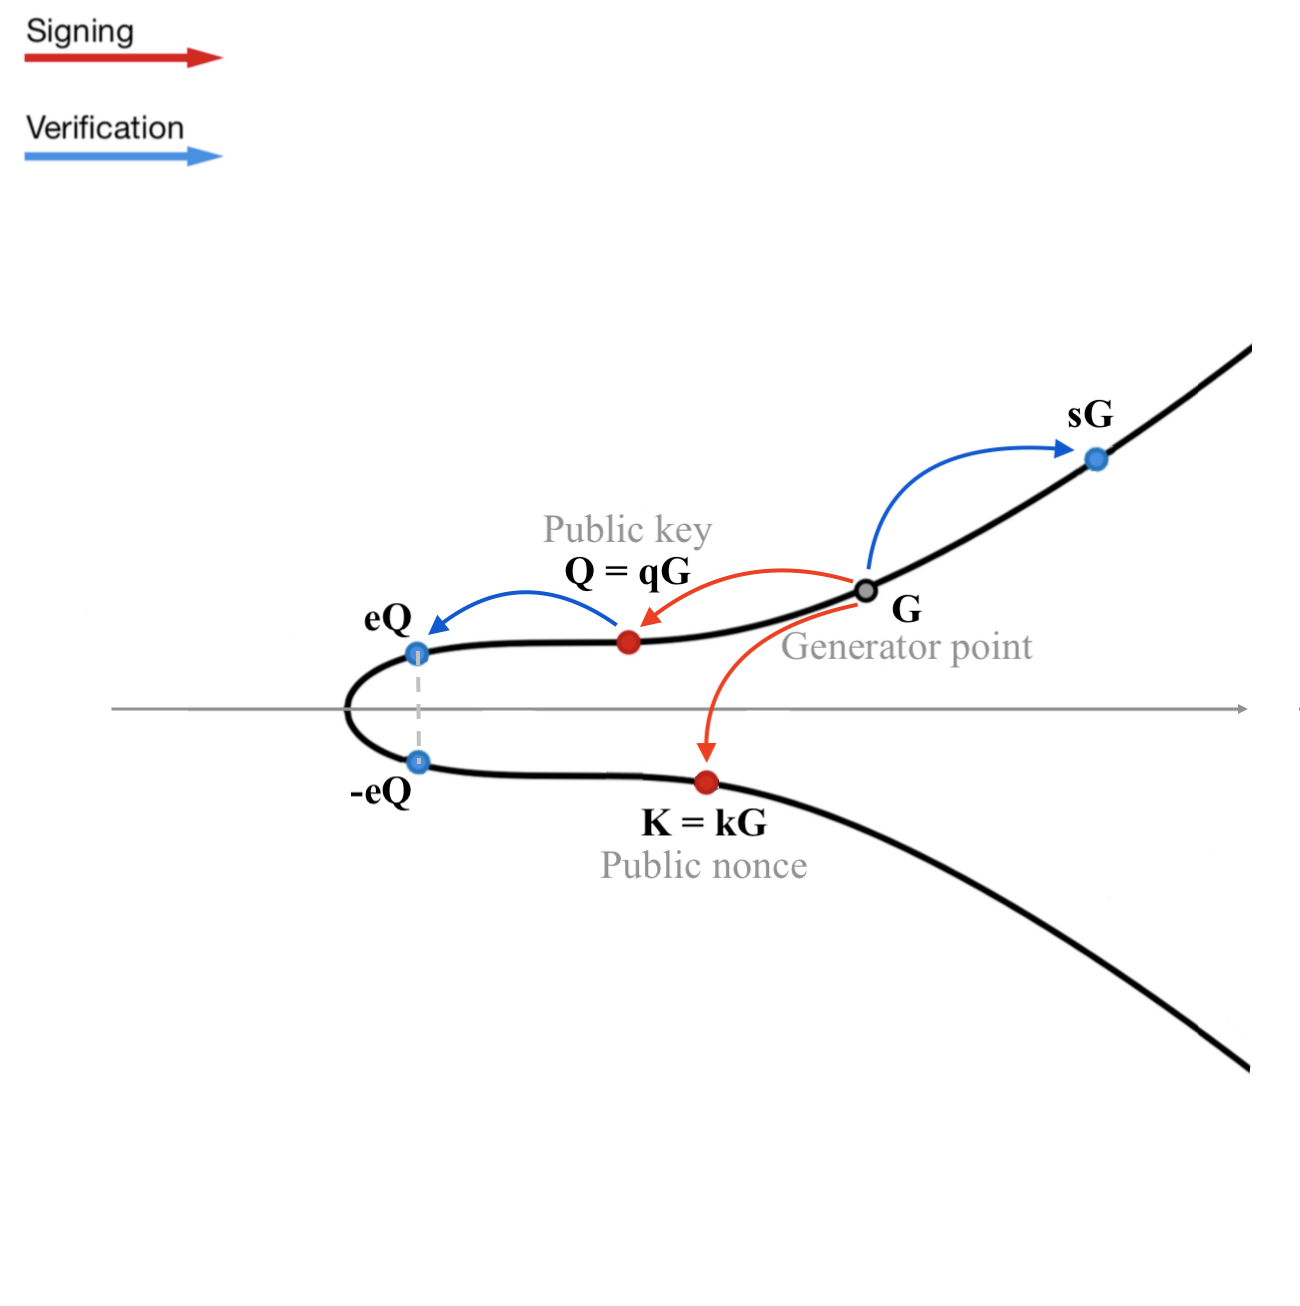
\includegraphics[scale=0.28]{images/Schnorr6}
						\source{\tiny \url{https://medium.com/cryptoadvance/how-schnorr-signatures-may-improve-bitcoin-91655bcb4744}}}
					\only<6> {\vspace*{-0.7cm}
						\hspace*{-0.9cm}
						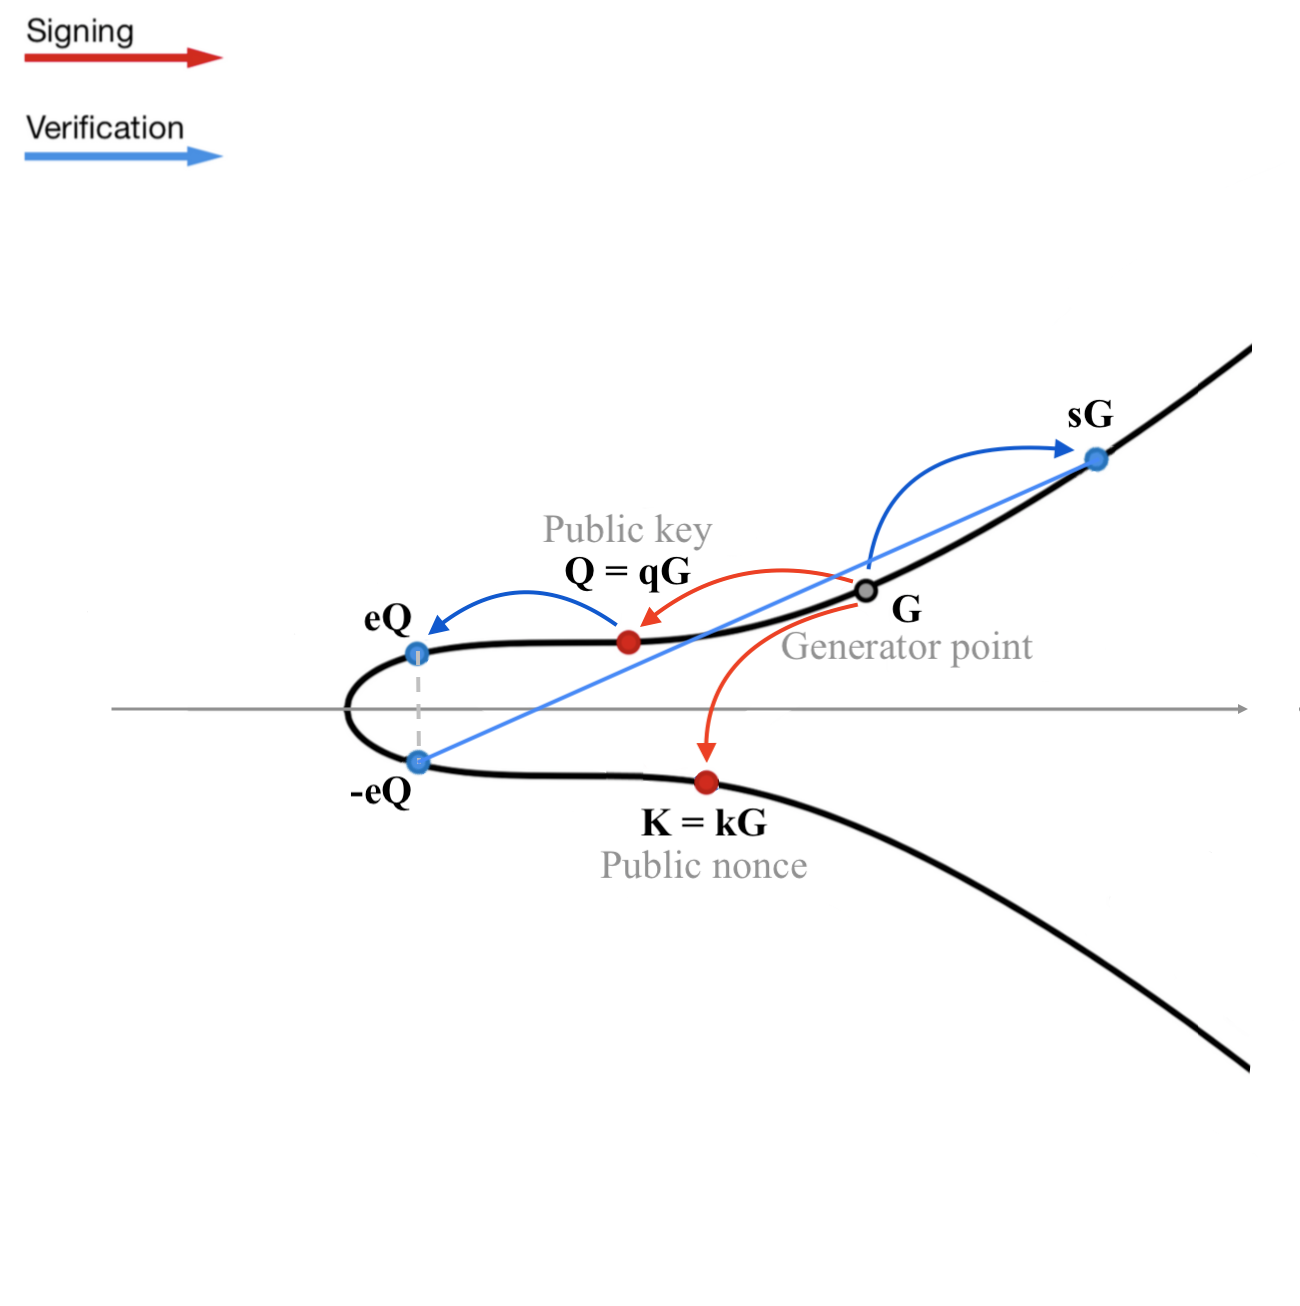
\includegraphics[scale=0.28]{images/Schnorr7}
						\source{\tiny \url{https://medium.com/cryptoadvance/how-schnorr-signatures-may-improve-bitcoin-91655bcb4744}}}
					\only<7-9> {\vspace*{-0.7cm}
						\hspace*{-0.9cm}
						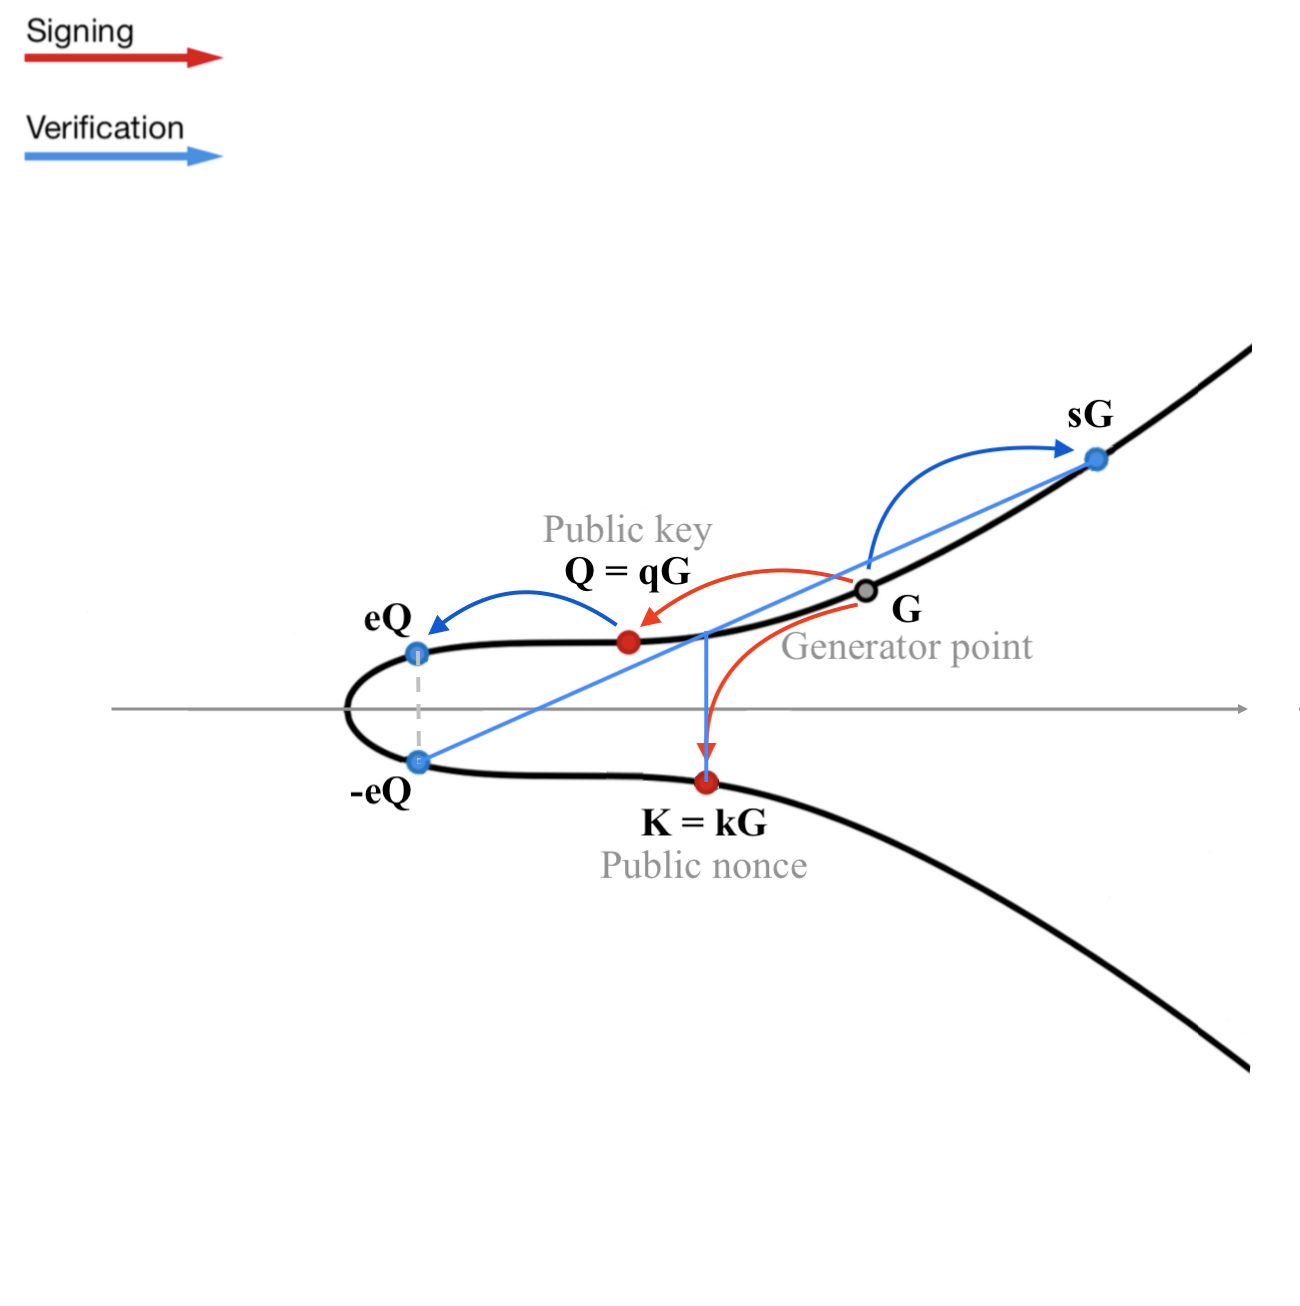
\includegraphics[scale=0.28]{images/Schnorr8}
						\source{\tiny \url{https://medium.com/cryptoadvance/how-schnorr-signatures-may-improve-bitcoin-91655bcb4744}}}
				\end{figure}
			\end{column}
		\end{columns}
	\end{frame}

	\begin{frame}{ECDSA vs. ECSSA}
		\begin{columns}
			\begin{column}{0.5\linewidth}
				ECDSA:
				\begin{itemize}
					\item<2 -> Malleable: given $(r, s)$ also $(r, -s \ (\text{mod} \ n))$ is a valid signature for same message and public key;
					\item<3 -> DER encoding: variable length, up to 73 bytes;
					\item<4 -> Cannot be validate faster in batch;
					\item<5 -> Requires the calculation of modular inverses;
					\item<6 -> Not linear: very complex higher level constructions.
				\end{itemize}
			\end{column}
			\begin{column}{0.5\linewidth}
				ECSSA:
				\begin{itemize}
					\item<2 -> Provably secure (SUF-CMA) in the Random Oracle Model assuming the ECDLP is hard $\Longrightarrow$ not malleable;
					\item<3 -> New encoding: fixed length, always 64 bytes;
					\item<4 -> Batch validation scales logarithmically;
					\item<5 -> No computational heavy operations involved;
					\item<6 -> Linear: easier higher level constructions.
				\end{itemize}
			\end{column}
		\end{columns}
	\end{frame}

	\subsubsection{Batch validation}
	\begin{frame}{Batch validation}
		A signature $(K, s)$ is valid if $K = sG - \text{hash}(x_K \ || \ Q \ || \ m)Q$. Thus, two valid signatures $(K_0, s_0)$ and $(K_1, s_1)$ satisfies:
		$$K_0 + K_1 = (s_0 + s_1)G - \text{hash}(x_{K_0} \ || \ Q_0 \ || \ m_0)Q_0 - \text{hash}(x_{K_1} \ || \ Q_1 \ || \ m_1)Q_1.$$
		Insecure: introduction of random factors.
		$$a_0K_0 + a_1K_1 =$$ $$
		= (a_0s_0 + a_1s_1)G - a_0\text{hash}(x_{K_0} \ || \ Q_0 \ || \ m_0)Q_0 - a_1\text{hash}(x_{K_1} \ || \ Q_1 \ || \ m_1)Q_1.$$
	\end{frame}

	\begin{frame}{Batch validation - Bos-Coster's algorithm}
		\begin{columns}
			\begin{column}{0.5\linewidth}
				$\ \ \ \ \ \ \ \ \ \ a_0K_0 + a_1K_1 =$ \\ $= (a_0 - a_1)K_0 + a_1(K_0 + K_1)$.
				
				\bigskip
				
				\pause
				\begin{itemize}
					\item<2 -> Sort the tuples according to $a_i$ in descending order;
					\item<3 -> While the list has length larger than one:
					\begin{itemize}
						\item<4 ->Substitute $(a_0, K_0)$ and $(a_1, K_1)$ with $(a_0 - a_1, K_0)$ and $(a_1, K_0 + K_1)$;
						\item<5 -> Sort the list again;
					\end{itemize}
					\item<6 -> When only one element remains, with very large probability it will be of the form $(1, K)$, otherwise it will be of the form $(a, K)$.
				\end{itemize}
			\end{column}
			\begin{column}{0.5\linewidth}
				\hspace*{0cm}
				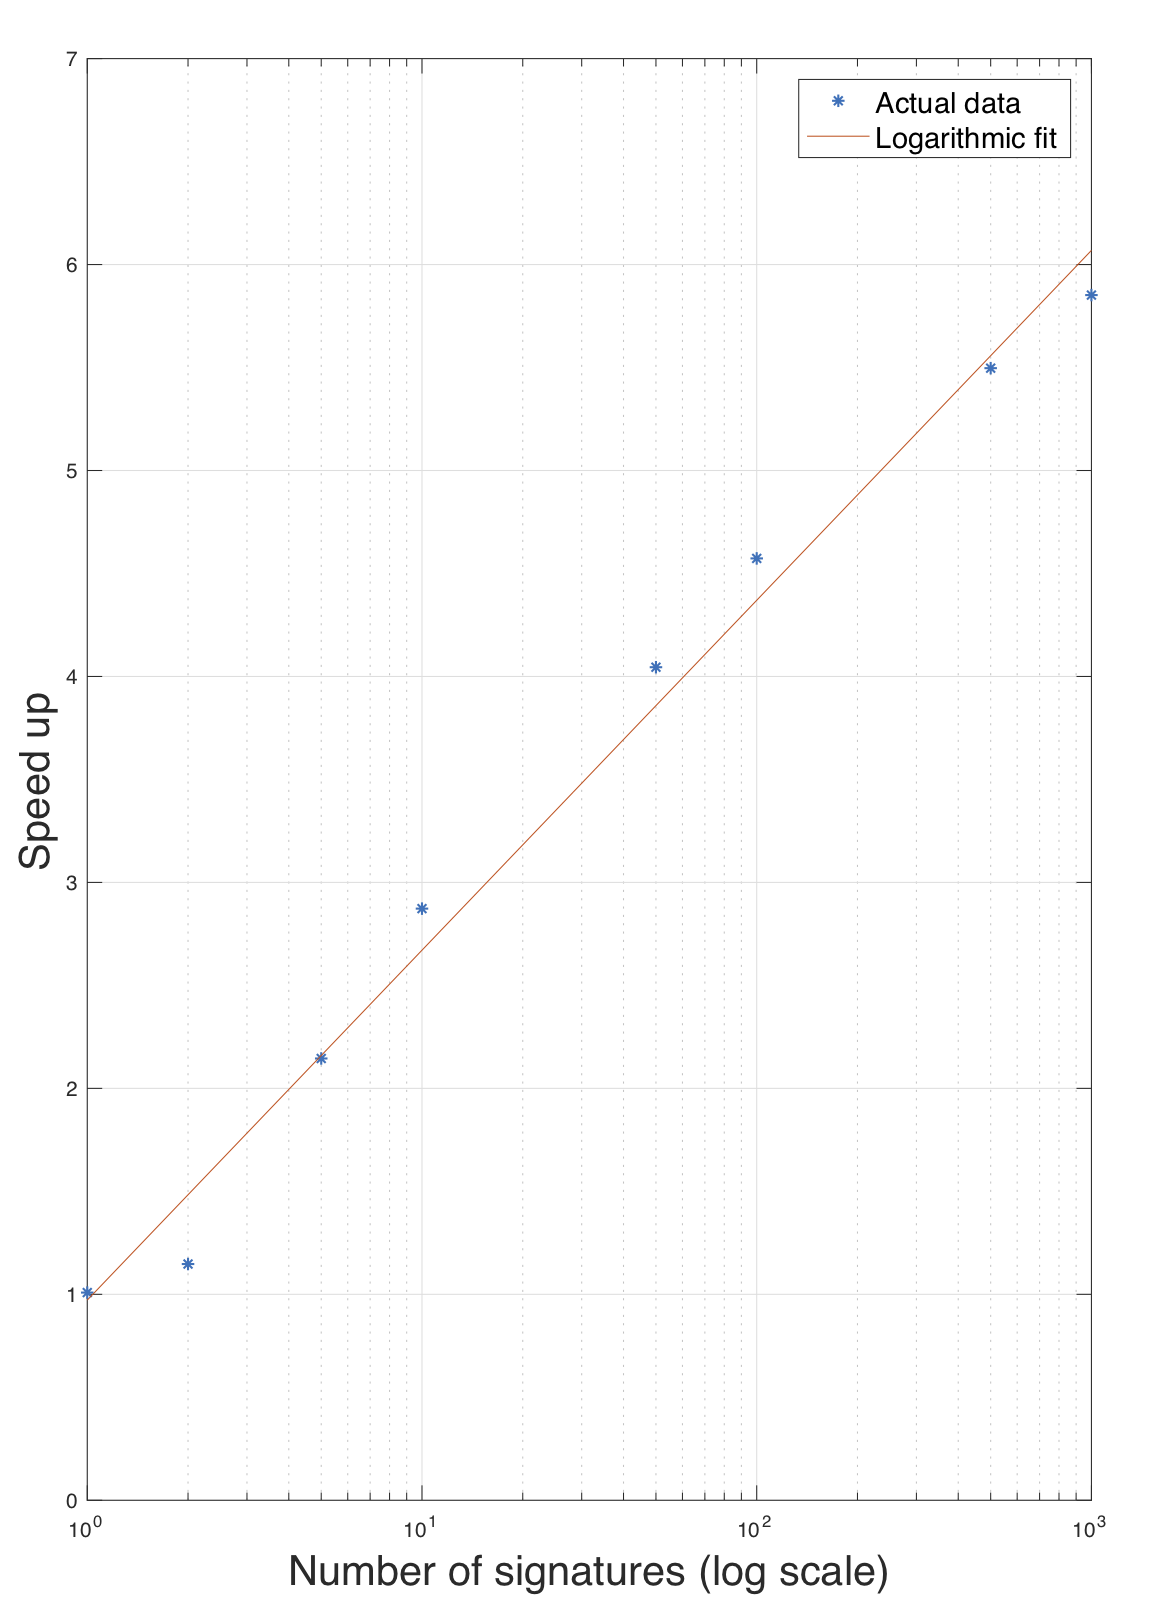
\includegraphics[scale=0.31]{images/speedup}
			\end{column}
		\end{columns}
	\end{frame}
	
	\section{ECSSA applications}
	
	\subsection{MuSig}
	\begin{frame}{Multi-signature schemes}
		Multi-signature schemes allow a group of users to cooperate to sign a single message: they are fundamental in real life applications.
		
		\bigskip
		\noindent
		\onslide<2 ->{Bitcoin multi-signature ($t$-of-$m$) is implemented naively:
		\begin{itemize}
			\item<3 -> Locking script: t $<$pubKey1$>$ $<$pubKey2$>$ ... $<$pubKeym$>$ \hphantom{em} \hphantom{em} \hphantom{em} \hphantom{ipsem}m
			OP\_CHECKMULTISIG
			\item<4 -> Unlocking script: 0 $<$sig1$>$ $<$sig2$>$ ... $<$sigt$>$
		\end{itemize}}
	
		\bigskip
		\noindent
		
%		\onslide<5-10>{\only<5-9>{Schnorr multi-signature (2-of-2) implemented naively:}
%			\only<10>{\sout{Schnorr multi-signature (2-of-2) implemented naively:}}
%		\begin{itemize}
%			\item<6-10>\only<6-9>{Alice ($\{q_A, Q_A\}$) and Bob ($\{q_B, Q_B\}$) generates $K_A$ and $K_B$;}\only<10>{\sout{Alice ($\{q_A, Q_A\}$) and Bob ($\{q_B, Q_B\}$) generates $K_A$ and $K_B$;}}
%			\item<7-10>\only<7-9>{They exchange them and set the public nonce at $K = K_A + K_B$. The joint public key is set at $Q = Q_A + Q_B$;}\only<10>{\sout{They exchange them and set the public nonce at $K = K_A + K_B$. The joint public key is set at $Q = Q_A + Q_B$;}}
%			\item<8-10>\only<8-9>{Their partial signatures are: $s_i = k_i + \text{hash}(x_K || Q || m)q_i, \ i \in \{A, B\}$;}\only<10>{\sout{Their partial signatures are: $s_i = k_i + \text{hash}(x_K || Q || m)q_i, \ i \in \{A, B\}$;}}
%			\item<9-10>\only<9>{The signature $(x_K, s_A + s_B)$ is valid on $m$ for public key $Q$.}\only<10>{\sout{The signature $(x_K, s_A + s_B)$ is valid on $m$ for public key $Q$.}}
%		\end{itemize}}

		\onslide<5-10>{\alert<10>{Schnorr multi-signature (2-of-2) implemented naively:}
		\begin{itemize}
			\item<6-10>\alert<10>{Alice ($\{q_A, Q_A\}$) and Bob ($\{q_B, Q_B\}$) generates $K_A$ and $K_B$;}
			\item<7-10>\alert<10>{They exchange them and set the public nonce at $K = K_A + K_B$. The joint public key is set at $Q = Q_A + Q_B$;}
			\item<8-10>\alert<10>{Their partial signatures are: $s_i = k_i + \text{hash}(x_K || Q || m)q_i, \ i \in \{A, B\}$;}
			\item<9-10>\alert<10>{The signature $(x_K, s_A + s_B)$ is valid on $m$ for public key $Q$.}
		\end{itemize}}
		\onslide<10>{\huge \centering \textcolor{red}{INSECURE: rogue key attack!}}
	\end{frame}

	\begin{frame}{MuSig: compact $m$-of-$m$ signature scheme}
		\begin{columns}
			\begin{column}{0.5\linewidth}
				\only<1-18>{
				MuSig($m, q_1, \langle L \rangle$):
				\begin{enumerate}
					\item<2 -> \textbf{for} $i \gets 1, m$ \textbf{do}:
					\begin{enumerate}
						\item<2 -> $a_i \gets \text{hash}(\langle L\rangle || Q_i)$;
					\end{enumerate}
					\item<3 -> $Q \gets \sum_{i = 1}^{m} a_iQ_i$;
					\item<4 -> $k_1 \xleftarrow{\text{\$}} \{1, ..., n - 1\}$;
					\item<5 -> $K_1 \gets k_1G, \ t_1 \gets \text{hash}(K_1)$;
					\item<6 -> \textbf{send} $t_1, K_1$;
					\item<11 -> $K \gets \sum_{i = 1}^{m} K_i$;
					\item<13 -> $c \gets \text{hash}(x_K || Q || m)$;
					\item<14 -> $s_1 \gets k_1 + ca_1q_1 \ (\text{mod} \ n)$;
					\item<15 -> \textbf{send} $s_1$;
					\item<17 -> $s \gets \sum_{i = 1}^{m} s_i \ (\text{mod} \ n)$;
					\item<18 -> \textbf{return} $(x_K , s)$.
				\end{enumerate}
			}
			\only<19-21>
			{
			MuSig ($\mu\Sigma$):
			\begin{itemize}
				\item<19-21> Compact: same size as the single user case;
				\item<20-21> Secure in the plain public key model: cross input aggregation at transaction level;
				\item<21> Key aggregation: signature indistinguishable from the single user case.
			\end{itemize}
			}
			\end{column}
			\begin{column}{0.62\linewidth}
				\begin{center}
					\begin{tikzpicture}[
						every node/.style = {% is not necessary, default node's shape is rectangle
						align=center}
						]
			
			
						\onslide<1-> {\node (a) {
\includegraphics[scale=0.17]{images/Alice.jpg}};}
						\onslide<1-> {\node (b) [text width=3cm, below=of a, yshift=1cm] {1: Alice};}
			
						\onslide<1-> {\node (d) [right=of a] {
\includegraphics[scale=0.22]{images/Bob.jpg}};}
						\onslide<1-> {\node (e) [text width=3cm, below=of d, yshift=1cm] {2: Bob};}
			
						\onslide<1-> {\node (g) [below=of a, xshift=2cm] {
\includegraphics[scale=0.1717]{images/Charlotte.jpg}};}
						\onslide<1-> {\node (h) [text width=3cm, below=of g, yshift=1cm] {3: Charlotte};}
						
						\only<2>{\node (i) [right=of a, xshift=-1.5cm, yshift=0.5cm] {$a_1, a_2$}};
						\only<3>{\node (i) [right=of a, xshift=-1.5cm, yshift=0.5cm] {$Q$}};
						\only<4>{\node (i) [right=of a, xshift=-1.5cm, yshift=0.5cm] {$k_1$}};
						\only<5>{\node (i) [right=of a, xshift=-1.5cm, yshift=0.5cm] {$K_1, t_1$}};
						\only<6>{\draw[->] (a) -- (d);
							\draw [->] (a) -- (g);};
						\only<6>{\node (i) [right=of a, xshift=-0.8cm, yshift=0.3cm] {$t_1$}};
						\only<6>{\node (i) [below=of a, xshift=1.2cm, yshift=0.9cm] {$t_1$}};
						\only<7>{\draw[->] (d) -- (a);
							\draw [->] (g) -- (a);};
						\only<7>{\node (i) [right=of a, xshift=-0.8cm, yshift=0.3cm] {$t_2$}};
						\only<7>{\node (i) [below=of a, xshift=1.2cm, yshift=0.9cm] {$t_3$}};
						\only<8>{\draw[->] (a) -- (d);
							\draw [->] (a) -- (g);};
						\only<8>{\node (i) [right=of a, xshift=-0.8cm, yshift=0.3cm] {$K_1$}};
						\only<8>{\node (i) [below=of a, xshift=1.2cm, yshift=0.9cm] {$K_1$}};
						\only<9>{\draw[->] (d) -- (a);
							\draw [->] (g) -- (a);};
						\only<9>{\node (i) [right=of a, xshift=-0.8cm, yshift=0.3cm] {$K_2$}};
						\only<9>{\node (i) [below=of a, xshift=1.2cm, yshift=0.9cm] {$K_3$}};
						\only<10>{\node (i) [right=of a, xshift=-1.7cm, yshift=1cm] {\small $t_2 \stackrel{?}{=} \text{hash}(K_2)$}};
						\only<10>{\node (i) [right=of a, xshift=-1.7cm, yshift=0.5cm] {\small $t_3 \stackrel{?}{=} \text{hash}(K_3)$}};
						\only<11>{\node (i) [right=of a, xshift=-1.5cm, yshift=0.5cm] {$K$}};
						\only<12>{\node (i) [right=of a, xshift=-2cm, yshift=1cm] {\small \textbf{if} $\text{jacobi}(y_K) \neq 1$:}};
						\only<12>{\node (i) [right=of a, xshift=-2cm, yshift=0.5cm] {\small $\ \ \ k_1 \gets n - k_1$}};
						\only<13>{\node (i) [right=of a, xshift=-1.5cm, yshift=0.5cm] {$c$}};
						\only<14>{\node (i) [right=of a, xshift=-1.5cm, yshift=0.5cm] {$s_1$}};
						\only<15>{\draw[->] (a) -- (d);
							\draw [->] (a) -- (g);};
						\only<15>{\node (i) [right=of a, xshift=-0.8cm, yshift=0.3cm] {$s_1$}};
						\only<15>{\node (i) [below=of a, xshift=1.2cm, yshift=0.9cm] {$s_1$}};
						\only<16>{\draw[->] (d) -- (a);
							\draw [->] (g) -- (a);};
						\only<16>{\node (i) [right=of a, xshift=-0.8cm, yshift=0.3cm] {$s_2$}};
						\only<16>{\node (i) [below=of a, xshift=1.2cm, yshift=0.9cm] {$s_3$}};
						\only<17>{\node (i) [right=of a, xshift=-1.5cm, yshift=0.5cm] {$s$}};
						\only<18>{\node (i) [right=of a, xshift=-1.5cm, yshift=0.5cm] {$(x_K, s)$}};
					\end{tikzpicture}
				\end{center}
			\end{column}
		\end{columns}
	\end{frame}

	\subsection{Threshold signature scheme}
	\begin{frame}{Threshold signature scheme ($t$-of-$m$)}
		\begin{columns}
			\begin{column}{0.51\linewidth}
				\begin{textblock*}{6cm}(1.3cm,1.1cm) 
					\only<1->{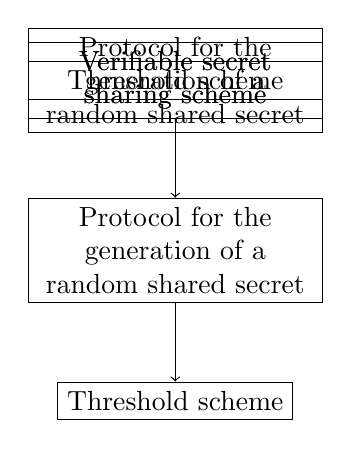
\begin{tikzpicture}[
						every node/.style = {% is not necessary, default node's shape is rectangle
							align=center}
						]	
						
						\node () at (0,0) {};
						\onslide<1-3>{\node[align = center, draw, text width=3.5cm] (a) {Verifiable secret sharing scheme};}
						\onslide<2-3>{\node[align = center, draw, below=of a, text width=3.5cm] (b) {Protocol for the generation of a random shared secret};}
						\onslide<3>{\node[align = center, draw,, below=of b] (c) {Threshold scheme};}
						
						
						\onslide<2-3>{\draw[->] (a) -- (b);}
						\onslide<3>{\draw[->] (b) -- (c);}
						
						\onslide<4-12>{\node[align = center, draw, text width=3.5cm] (a) {Verifiable secret sharing scheme};}
						\onslide<13-17>{\node[align = center, draw, text width=3.5cm] (a) {Protocol for the generation of a random shared secret};}
						\onslide<18-23>{\node[align = center, draw, text width=3.5cm] (a) {Threshold scheme};}
						\end{tikzpicture}}
				\end{textblock*}
				\begin{textblock*}{6cm}(0.3cm,2.5cm) 
					\only<4-9>{
						The dealer:
						\only<5-6>{
							\begin{itemize}
								\item<5-6> {generates secret $s$ and $s' \xleftarrow{\text{\$}} \{1, ..., n - 1\}$;}
								\item<6> {commits to them through the Pedersen commitment $C_0 = sG + s'H$: $C_0$ is broadcast.}
						\end{itemize}}
						\only<7->{
							\begin{itemize}
								\item<7-> {chooses random polynomials:\\
									$f(u) = s + f_1u + ... + f_{t - 1}u^{t - 1}$,\\
									$f'(u) = s' + f_1'u + ... + f_{t - 1}'u^{t - 1}$,\\
									$f_j, \ f_j' \xleftarrow{\text{\$}} \{1, ..., n - 1\}$;}
								\item<8-> computes $(s_i, s_i') = (f(i) \ (\text{mod \ n}), f'(i) \ (\text{mod \ n}))$, \\ $i \in \{1, ..., m\}$ and sends them secretly to $P_i$;
								\item<9-> broadcasts the commitment to the sharing polynomials: $C_j = f_jG + f_j'H$,\\ $j \in \{1, ..., t - 1\}$.
						\end{itemize}}
					}
					\only<10-12>{
					The participants:
					\only<11-12>{
						\begin{itemize}
							\item<11-> verify the consistency of their shares of secret: $s_iG + s_i'H = \sum_{j = 0}^{t - 1}i^jC_j$;
							\item<12-> to reconstruct the secret they rely on Lagrange's interpolation formula: \\
							$f(u) = \sum_{i} f(i)\omega_i(u)$, where $\omega_i(u) = \prod_{j \neq i} \frac{u - j}{i - j} \ (\text{mod} \ n)$.
							\\
							$s = f(0) = \sum_{i}s_i\omega_i$, with $\omega_i = \omega_i(0) = \prod_{j \neq i} \frac{j}{j - i} \ (\text{mod} \ n)$.
						\end{itemize}
					}
					}
				\end{textblock*}
				\begin{textblock*}{6cm}(0.3cm,2.8cm) 
					\only<13-17>{
					Each participant:
					\only<14-17>{
					\begin{itemize}
						\item<14-17> acts as the dealer in the previous protocol ($f_i(u) = \sum_{j = 0}^{t - 1}a_{ij}u^j$, $a_{i0} = r_i$);
						\item<16-17> the shared secret is $r = \sum_{i = 1}^{m}r_i \ (\text{mod} \ n)$ with shares $s_i = \sum_{j = 1}^{m} f_j(i) \ (\text{mod} \ n)$;
						\item<17> broadcast his share of the public key $R_j = r_jG$ ($R = \sum_{j = 1}^{m}R_j = \sum_{j = 1}^{m}r_jG = rG$).
					\end{itemize}
					}
				}
			\end{textblock*}
			\begin{textblock*}{6cm}(0.3cm,2.2cm) 
				\only<18-19>{
					After having established a distributed key pair $(\alpha_1, ..., \alpha_m) \xleftrightarrow{\text{(t, m)}} (q|Q)$ through the protocol for the generation of a random shared secret (that acts as key generation protocol) the signers:
					\only<18-19>{
						\begin{itemize}
							\item<19> run again the same protocol to produce a nonces pair: $(\beta_1, ..., \beta_m) \xleftrightarrow{\text{(t, m)}} (k|K)$.
						\end{itemize}
				}
			}
				\only<20-23>{
				Then each signer $i$:
				\begin{itemize}
					\item<20-23> checks whether $\text{jacobi}(y_K) \neq 1$; if it is the case she sets $\beta_i = n - \beta_i$;
					\item<21-23> reveals her partial signature: $\gamma_i  = \beta_i + e\alpha_i \ (\text{mod} \ n)$, with $e = \text{hash}(x_K||Q||msg)$;
					\item<22-23> computes $\sigma = \sum_{j = 1}^{t} \gamma_j\omega_j \ (\text{mod} \ n)$, with $\omega_j = \prod_{h \neq j} \frac{h}{h - j} \ (\text{mod} \ n)$: $\sigma$ is such that $\sigma = k + eq \ (\text{mod} \ n)$;
					\item<23> the signature is $(x_K, \sigma)$.
				\end{itemize}
			
			}
			\end{textblock*}
		
			\end{column}
			\begin{column}{0.65\linewidth}
				\begin{tikzpicture}[
					every node/.style = {% is not necessary, default node's shape is rectangle
					align=center}
					]	
				
					\node () at (0,0) {};
					\onslide<1-17> {\node(a) [yshift=2cm] {
\includegraphics[scale=0.16]{images/Alice.jpg}};}
					\onslide<1-3> {\node (b) [text width=3cm, above=of a, yshift=-1cm, xshift=-0.1cm] {Alice};}
					\onslide<4-12> {\node (b) [text width=3cm, above=of a, yshift=-1cm, xshift=-0.1cm] {Dealer: Alice};}
					\onslide<13-17> {\node (b) [text width=3cm, above=of a, yshift=-1cm, xshift=-0.1cm] {1: Alice};}
					\only<18-23> {\node(a) [yshift=2cm] {
\includegraphics[scale=0.16]{images/Alice.jpg}};}
					\only<18-23> {\node (b) [text width=3cm, above=of a, yshift=-1cm, xshift=-0.1cm] {1: Alice};}
					
					\onslide<1-17> {\node (d) [below=of a, xshift = -1.75cm] {
\includegraphics[scale=0.21]{images/Bob.jpg}};}
					\onslide<1-3> {\node (e) [text width=3cm, below=of d, yshift=1cm, xshift=0.2cm] {Bob};}
					\onslide<4-12> {\node (e) [text width=3cm, below=of d, yshift=1cm, xshift=0.2cm] {1: Bob};}
					\onslide<13-17> {\node (e) [text width=3cm, below=of d, yshift=1cm, xshift=0.2cm] {2: Bob};}
					
					\onslide<1-17> {\node (g) [below=of a, xshift=1.75cm] {
\includegraphics[scale=0.16]{images/Charlotte.jpg}};}
					\onslide<1-3> {\node (h) [text width=3cm, below=of g, yshift=1cm] {Charlotte};}
					\onslide<4-12> {\node (h) [text width=3cm, below=of g, yshift=1cm] {2: Charlotte};}
					\onslide<13-17> {\node (h) [text width=3cm, below=of g, yshift=1cm] {3: Charlotte};}
					\only<18-23> {\node (g) [below=of a] {
\includegraphics[scale=0.16]{images/Charlotte.jpg}};}
					\only<18-23> {\node (h) [text width=3cm, below=of g, yshift=1cm] {3: Charlotte};}
					
					\only<5> {\node [right=of a, xshift=-1.45cm, yshift=0.5cm] {$s, s'$};}
					\only<6>{\draw[->] (a) -- (d);
						\draw [->] (a) -- (g);
					    \node [right=of a, xshift=-1.5cm, yshift=-1.7cm] {$C_0$};
				    	\node [right=of a, xshift=-3.8cm, yshift=-1.7cm] {$C_0$};};
					\only<7> {\node [right=of a, xshift=-1.45cm, yshift=0.5cm] {$f, f'$};}
					\only<8>{\draw[->] (a) -- (d);
						\draw [->] (a) -- (g);
						\node [right=of a, xshift=-1.5cm, yshift=-1.7cm] {$(s_2, s_2')$};
						\node [right=of a, xshift=-4.5cm, yshift=-1.7cm] {$(s_1, s_1')$};}
					\only<9>{\draw[->] (a) -- (d);
						\draw [->] (a) -- (g);
						\node [right=of a, xshift=-1.5cm, yshift=-1.7cm] {$C_j$};
						\node [right=of a, xshift=-3.8cm, yshift=-1.7cm] {$C_j$};};
					\only<11> {\node [above=of d, xshift=1.75cm, yshift=-1.6cm] {
\includegraphics[scale=0.07]{images/pensiero.jpg}};}
					\only<12>{\draw [->] (d) -- (g);
						\draw [->] (g) -- (d);
						\node [right=of d, xshift=-0.8cm, yshift=0.3cm] {$s$};};
					
					\only<14-15>{\node [right=of a, xshift=-1.4cm, yshift=0.3cm] {$r_1, f_1$};
									\node [right=of d, xshift=-1.5cm, yshift=0.3cm] {$r_2, f_2$};
									\node [right=of g, xshift=-1.4cm, yshift=0.3cm] {$r_3, f_3$};};
					\only<15>{\draw [->] (a) -- (d);
									 \draw [->] (d) -- (a);
									 \draw [->] (a) -- (g);
									 \draw [->] (g) -- (a);
									 \draw [->] (d) -- (g);
									 \draw [->] (g) -- (d);};
					\only<16>{\node [right=of a, xshift=-1.4cm, yshift=0.3cm] {$s_1$};
						\node [right=of d, xshift=-1.5cm, yshift=0.3cm] {$s_2$};
						\node [right=of g, xshift=-1.4cm, yshift=0.3cm] {$s_3$};};		 
					\only<17>{\draw [->] (a) -- (d);
						\draw [->] (d) -- (a);
						\draw [->] (a) -- (g);
						\draw [->] (g) -- (a);
						\draw [->] (d) -- (g);
						\draw [->] (g) -- (d);
						\node [right=of a, xshift=-1.5cm, yshift=-1.7cm] {$R_1$};
						\node [right=of a, xshift=-3.9cm, yshift=-1.7cm] {$R_1$};
						\node [right=of a, xshift=-3.25cm, yshift=-1.8cm] {$R_2$};
						\node [right=of a, xshift=-2.1cm, yshift=-1.8cm] {$R_3$};
						\node [right=of d, xshift = -0.9cm, yshift = 0.3cm] {$R_2$};
						\node [left=of g, xshift = 0.9cm, yshift = -0.3cm] {$R_3$};
					};
				\only<18>{\node [right=of a, xshift=-1.4cm, yshift=0.3cm] {$\alpha_1$};
					\node [right=of g, xshift=-1.4cm, yshift=0.3cm] {$\alpha_3$};
				\draw [->] (a) -- (g);
				\draw [->] (g) -- (a);}
				\only<19>{\node [right=of a, xshift=-1.4cm, yshift=0.3cm] {$\alpha_1, \beta_1$};
					\node [right=of g, xshift=-1.4cm, yshift=0.3cm] {$\alpha_3, \beta_3$};
				\draw [->] (a) -- (g);
				\draw [->] (g) -- (a);}
				\only<21>{
					\draw[transform canvas={xshift=1em}, ->] (a) -- (g);
					\draw[transform canvas={xshift=-1em}, ->] (g) -- (a);
					\node [right=of a, xshift=-2cm, yshift=-2cm] {$\gamma_1$};
					\node [right=of g, xshift=-3.2cm, yshift=2cm] {$\gamma_3$};}
				\only<22>{
					\node [right=of a, xshift=-1.4cm, yshift=0.3cm] {$\sigma$};
					\node [right=of g, xshift=-1.4cm, yshift=0.3cm] {$\sigma$};}
				\only<23>{
					\node [right=of a, xshift=-1.4cm, yshift=0.3cm] {$(x_K, \sigma)$};
					\node [right=of g, xshift=-1.4cm, yshift=0.3cm] {$(x_K, \sigma)$};}
				\end{tikzpicture}
			\end{column}
		\end{columns}
	\end{frame}

	\begin{frame}{ECDSA vs. ECSSA (multi-signature)}
		ECDSA:
		\begin{itemize}
			\item Locking script: t $<$pubKey1$>$ $<$pubKey2$>$ ... $<$pubKeym$>$ \hphantom{em} \hphantom{em} \hphantom{em} \hphantom{ipsem}m
			OP\_CHECKMULTISIG
			\item Unlocking script: 0 $<$sig1$>$ $<$sig2$>$ ... $<$sigt$>$
		\end{itemize}
		
		\bigskip
		\noindent
		\onslide<2>{
		ECSSA:
		\begin{itemize}
			\item Locking script: $<$jointPubKey$>$ OP\_SCHNORR
			\item Unlocking script: $<$jointSig$>$
		\end{itemize}}
	\end{frame}

	\subsection{Adaptor signatures}
	\begin{frame}{Adaptor signatures}
		Building block for \textit{scriptless script}: aim at encapsulating the flexibility of script semantics in fixed size signatures.
		
		\bigskip
		\noindent
		\onslide<2->{How?}
		\onslide<3->{The idea is to add to the public nonce $K$ a random $T = tG$ but still consider $k$ as private nonce: this results in an invalid signature, however learning $t$ is equivalent to learning a valid signature.}
		
		\bigskip
		\noindent
		\onslide<4->{If $t$ is some necessary data for the execution of a separate protocol, arbitrary steps of arbitrary protocols can be made equivalent to signature production.}
	\end{frame}

	\begin{frame}{Cross-chain atomic swaps}
		Exchange of different crypto-currencies among two distrustful users in an atomic and decentralized way.
		
		\bigskip
		\noindent
		\onslide<2->{This is done via Hashed TimeLock Contract (HTLC), special locking scripts that ensures the atomicity of the transactions on both blockchains.}
		
		\bigskip
		\noindent
		\onslide<3->{
			OP\_IF
\\
			\ \ \ \ \ OP\_HASH256 $<$digest$>$ OP\_EQUALVERIFY OP\_DUP \\ 
			\ \ \ \ \ OP\_HASH160 $<$Bob address$>$ \\
			OP\_ELSE \\
			\ \ \ \ \ $<$num$>$ OP\_CHECKSEQUENCEVERIFY OP\_DROP \\ 
			\ \ \ \ \ OP\_DUP OP\_HASH160 $<$Alice addres$>$ \\
			OP\_ENDIF \\
			OP\_EQUALVERIFY OP\_CHECKSIG}
		
		\bigskip
		\noindent
		\onslide<4->{Easily identifiable (lack of privacy) and cumbersome (high fees).}
	\end{frame}

	\def\bitcoin{%
		\leavevmode
		\vtop{\offinterlineskip %\bfseries
			\setbox0=\hbox{B}%
			\setbox2=\hbox to\wd0{\hfil\hskip-.03em
				\vrule height .3ex width .15ex\hskip .08em
				\vrule height .3ex width .15ex\hfil}
			\vbox{\copy2\box0}\box2}}

	\begin{frame}{Cross-chain atomic swaps via adaptor signatures}
		\begin{tikzpicture}[
		every node/.style = {% is not necessary, default node's shape is rectangle
			align=center}
		]
		
		\onslide<1->{
		\node () at (0,0) {};
		\node (b1) [xshift = -2cm] {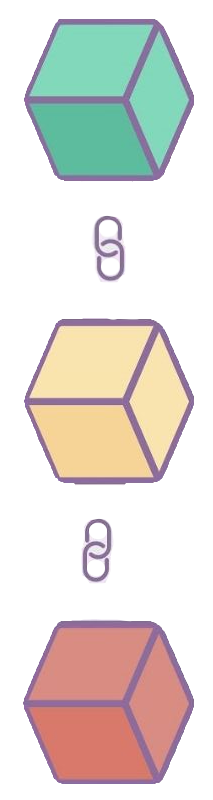
\includegraphics[scale=0.1]{images/blockchain.png}};
		
		\node (a) [right=of b1] {
\includegraphics[scale=0.15]{images/Alice.jpg}};
		\node (b) [text width=3cm, below=of a, yshift=1cm] {Alice};
		
		\node (d) [right=of a] {
\includegraphics[scale=0.2]{images/Bob.jpg}};
		\node (e) [text width=3cm, below=of d, yshift=1cm] {Bob};
		
		\node (b2) [right=of d] {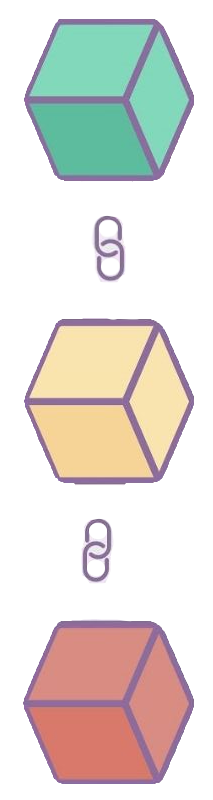
\includegraphics[scale=0.1]{images/blockchain.png}};
		
		\node (btc) [above=of b1, yshift = -1cm]{
\includegraphics[scale=0.05]{images/bitcoin.png}};
		\node (eth) [above=of b2, yshift = -1cm]{
\includegraphics[scale=0.05]{images/ethereum.png}};
		
		\only<2->{
		\node () [right=of a, xshift = -4.4cm, yshift=1cm] {$Q_A^{\small \bitcoin}, Q_A^{\tiny \mathsf{\Xi}}$};
		\node () [right=of d, xshift = -1.8cm, yshift=1cm] {$Q_B^{\small \bitcoin}, Q_B^{\tiny \mathsf{\Xi}}$};}
		\only<3->{
		\node () [right=of a, xshift = -1.7cm, yshift = 1.2cm] {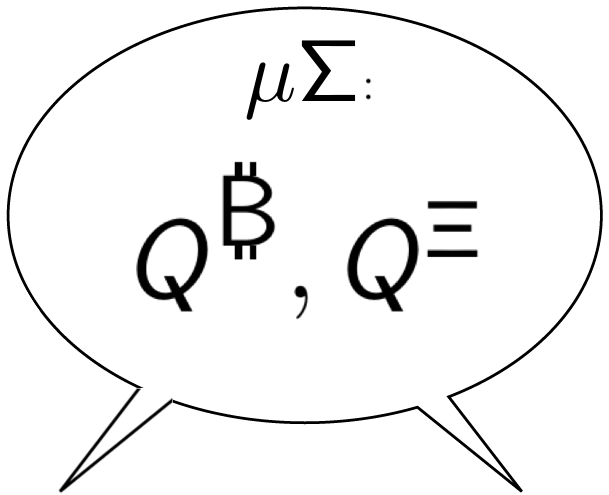
\includegraphics[scale=0.1]{images/fumetto.png}};
		}
		}
		
		\end{tikzpicture}
			
	\end{frame}
\end{document}
